\documentclass[a4paper,11pt]{report}

% ---- Page layout ----
\usepackage[margin=2.5cm]{geometry}

% ---- Fonts (XeLaTeX; needed for correct Vietnamese diacritics) ----
\usepackage{fontspec}

% ---- Typography & links ----
\usepackage{microtype}
\usepackage{xcolor}
\usepackage{hyperref}
\hypersetup{
    colorlinks = true,
    linkcolor  = blue!50!black,
    citecolor  = blue!50!black,
    urlcolor   = blue!50!black
}

% ---- Math ----
\usepackage{amsmath,amssymb,mathtools}

% ---- Figures & tables ----
\usepackage{graphicx}
\usepackage{float}
\usepackage{booktabs}
\usepackage{array}
\usepackage{caption}
\usepackage{subcaption}

% ---- Header / footer ----
\usepackage{fancyhdr}
\pagestyle{fancy}
\fancyhf{}
\rfoot{\thepage}
\renewcommand{\headrulewidth}{0pt}

\begin{document}

\begin{titlepage}
    \centering
    \vspace*{3cm}

    {\LARGE\bfseries Customer Retention \& Churn Prediction}\\[0.4cm]
    {\Large A Churn Prediction System for E-commerce Retention Marketing}\\[2cm]

    \rule{0.8\linewidth}{0.6pt}\\[0.5cm]
    {\large Business Data Analytics Project Report}\\[0.2cm]
    \rule{0.8\linewidth}{0.6pt}

    \vfill

    \begin{tabular}{ll}
        \textbf{Instructor:} & Nguyễn Bình Minh \\
    \end{tabular}

    \vspace{0.8cm}

    \textbf{Group Members}\\[0.3cm]
    \begin{tabular}{ll}
        Nguyễn Bá Anh & 20261218M \\
        Nguyễn Tiến Khương & 20261220M \\
        Nguyễn Trọng Huy Hoàng & 20251191M \\
        Nguyễn Tuệ Lâm & 20261207M \\
    \end{tabular}

    \vspace{1cm}
    {\large \today}

    \vspace*{1cm}
\end{titlepage}

\tableofcontents

\chapter{Introduction}
\label{ch:introduction}
\section{Project Background}
\label{sec:1-1}

Retail businesses rely on customer relationships and repeat purchases to maintain sustainable revenue. However, customers may gradually reduce their purchasing activity or stop purchasing altogether.

Identifying these customers before they become inactive can be challenging, particularly when businesses have large customer bases and substantial transaction histories. Without an effective way to identify potential churn, businesses may miss opportunities to maintain customer relationships and encourage repeat purchases.

Customer churn prediction can help businesses better understand customer purchasing behavior and identify customers who may be at risk of becoming inactive.

\section{Problem Statement}
\label{sec:1-2}

\begin{itemize}
    \item \textbf{Difficulty in early identification of churn risk.} Retail businesses struggle to detect customers who are likely to stop purchasing based on historical transaction behavior. Traditional methods often identify inactive customers only after a long period of inactivity, by which time retention opportunities are already limited.
    \item \textbf{Limited retention resources impacting revenue growth.} The business needs to increase sales revenue but operates under constrained marketing and retention resources. Without a data-driven way to prioritize at-risk customers, retention efforts may be inefficient and fail to maximize revenue.
\end{itemize}

\section{Research Questions}
\label{sec:1-3}

\begin{enumerate}
    \item How can transaction history be converted into customer-level data for churn prediction?
    \item How well does purchasing behavior predict churn?
    \item Does churn-risk ranking improve prioritization under limited retention resources compared to rule-based targeting?
    \item Which customer behaviors are most associated with churn? (Correlation, not causation.)
\end{enumerate}

\section{Project Objectives}
\label{sec:1-4}

To develop a data-driven churn prediction model that identifies customers at risk of leaving based on their purchasing history, enabling retail e-commerce businesses to prioritize limited retention resources and maximize sales revenue.

\section{Scope and Limitations}
\label{sec:1-5}

\textbf{In scope:} existing-customer retention, churn prediction, customer snapshots, weekly batch scoring, risk ranking and Top-K targeting.

\textbf{Out of scope / not claimed:}
\begin{itemize}
    \item Causal uplift and incremental campaign revenue -- the transaction data contain no randomized treatment/control information.
    \item A live deployment. \textbf{Chapters~\ref{ch:deployment} and~\ref{ch:feedback} describe a proposed operational design}; they are not evaluated on a running system.
    \item Profit analysis based on real margins or costs -- these are not in the data and enter only as stated assumptions.
\end{itemize}

\section{Report Structure}
\label{sec:1-6}

The report is organized into ten chapters:

\begin{enumerate}
    \item \textbf{Introduction} -- background, problem statement, research questions, objectives and scope.
    \item \textbf{Problem Statement and Approach} (Chapter~\ref{ch:problem-approach}) -- the business problem, objectives and success criteria, and the analytical approach used to address them.
    \item \textbf{Dataset and Data Specification} (Chapter~\ref{ch:dataset}) -- the Online Retail II dataset, its characteristics and limitations, and its schema and conventions.
    \item \textbf{Data Understanding} (Chapter~\ref{ch:data-understanding}) -- exploratory analysis of sales, customers and purchasing behavior, and the feasibility of churn prediction.
    \item \textbf{Data Preparation} (Chapter~\ref{ch:data-preparation}) -- cleaning, customer snapshots, features, churn labels and the temporal split.
    \item \textbf{Modeling} (Chapter~\ref{ch:modeling}) -- baselines, feature sets, algorithms, tuning and interpretability.
    \item \textbf{Evaluation} (Chapter~\ref{ch:evaluation}) -- predictive, ranking and business-impact evaluation on the unseen test period.
    \item \textbf{Deployment} (Chapter~\ref{ch:deployment}) -- the proposed weekly scoring design.
    \item \textbf{Feedback} (Chapter~\ref{ch:feedback}) -- monitoring and retraining.
    \item \textbf{Conclusion} (Chapter~\ref{ch:conclusion}) -- summary, limitations and future work.
\end{enumerate}


\chapter{Problem Statement and Approach}
\label{ch:problem-approach}
\section{E-commerce Sales Business}
\label{sec:2-1}

The business sells products through an e-commerce transaction system, and sales generate revenue from customer purchases. At a high level:
\begin{equation*}
    \text{Profit} = \text{Sales Revenue} - \text{Business Costs}
\end{equation*}
Costs may include product/operating costs, marketing costs and retention incentive costs.

\section{Revenue from New and Existing Customers}
\label{sec:2-2}

Sales revenue can be generated by both new customers making their first purchases and existing customers making repeat purchases. New customers contribute to business growth by expanding the customer base, while existing customers may generate additional revenue through continued purchasing activity.

\section{Customer Churn as a Business Problem}
\label{sec:2-3}

When existing customers gradually reduce their purchasing activity or stop purchasing altogether, businesses may lose potential future sales. Understanding the behavior of these customers can help businesses identify opportunities to encourage repeat purchases.

\section{Retention and Marketing Cost Constraints}
\label{sec:2-4}

Retention activities require resources. The company cannot necessarily apply the same retention action to every existing customer because marketing budget, campaign capacity and incentives are limited. Retention resources must be allocated selectively.

\section{Business Objectives}
\label{sec:2-5}

The primary business objective is to support sustainable sales revenue by identifying existing customers who are at risk of churn and enabling more informed customer retention decisions. The specific objectives are:

\begin{itemize}
    \item \textbf{Identify at-risk customers:} recognize existing customers who are likely to stop purchasing within a predefined period.
    \item \textbf{Understand purchasing behavior:} investigate customer characteristics, such as purchase frequency, monetary value and time since the last purchase, that may be associated with churn risk.
    \item \textbf{Support customer prioritization:} provide insights that help the business prioritize customers for potential retention activities.
\end{itemize}

\section{Success Criteria}
\label{sec:2-6}

Success is defined \textbf{relative to simple alternatives} rather than by arbitrary absolute thresholds:

\begin{center}
\begin{tabular}{@{}p{3cm}p{11.5cm}@{}}
    \toprule
    Level & Criterion (evaluated on the unseen test period) \\
    \midrule
    Predictive & Final model PR-AUC exceeds the test-period churn rate (random reference) and the recency-rule baseline. \\
    Targeting & Final model Lift@K and Recall@K at the chosen operating $K$ (e.g.\ 20--30\%) exceed the recency-rule baseline, averaged over weekly scoring dates. \\
    Stability & Top-K performance does not collapse on individual test weeks (report mean $\pm$ standard deviation). \\
    Business scenario & Under the base scenario, estimated net impact at the chosen $K$ is positive and higher than for recency-rule and random targeting at the same $K$. \\
    \bottomrule
\end{tabular}
\end{center}

\section{From Business Objective to Analytical Problem}
\label{sec:2-7}

Increasing revenue requires more repeat-purchase revenue from existing customers and efficient use of retention resources. The analytical direction is therefore to identify existing customers at risk of not purchasing again, estimate churn probability, and prioritize customers for retention activities.

\section{Customer Retention Strategy}
\label{sec:2-8}

\begin{center}
\begin{tabular}{@{}c@{}}
    \textbf{Eligible Existing Customers} \\
    $\downarrow$ \\
    \textbf{Churn Prediction} -- estimate churn probability \\
    $\downarrow$ \\
    \textbf{Risk Ranking} -- rank customers by predicted churn risk \\
    $\downarrow$ \\
    \textbf{Business Rules and Available Capacity} \\
    $\downarrow$ \\
    \textbf{Target Customers for Retention} -- prioritize customers for potential campaigns \\
\end{tabular}
\end{center}

\section{Implementation Roadmap}
\label{sec:2-9}

The approach is implemented as a sequence of steps, each covered by one chapter:

\begin{itemize}
    \item \textbf{Understand the data} (Chapter~\ref{ch:data-understanding}) -- sales and customer behavior, purchase intervals and revenue by purchase cadence, which inform the prediction horizon $H$ and the activity threshold $R_{\max}$.
    \item \textbf{Prepare customer snapshots} (Chapter~\ref{ch:data-preparation}) -- turn transactions into Customer $\times$ Snapshot Date rows with point-in-time features, churn labels and an embargoed temporal split.
    \item \textbf{Model churn risk} (Chapter~\ref{ch:modeling}) -- compare baselines and algorithms and select a final model.
    \item \textbf{Evaluate} (Chapter~\ref{ch:evaluation}) -- predictive, ranking and scenario-based business-impact evaluation on the unseen test period.
    \item \textbf{Deploy} (Chapter~\ref{ch:deployment}) -- weekly batch scoring and Top-K targeting, as a proposed operational design.
\end{itemize}


\chapter{Dataset and Data Specification}
\label{ch:dataset}
\section{Data Source and Collection}
\label{sec:3-1}

The project uses the publicly available \textbf{Online Retail II} dataset as a historical extract of e-commerce transaction records. The dataset is obtained and loaded into the analytical environment for data inspection, preprocessing and customer churn analysis. It contains transaction-level information, including invoice identifiers, customer identifiers, product codes, quantities, prices and invoice dates.

\section{Dataset Characteristics and Limitations}
\label{sec:3-2}

The dataset covers the period from December 2009 to December 2011. Its relatively limited historical coverage constrains the number of customer snapshots and future observation periods available for churn labeling (Section~\ref{sec:5-9}). In addition, the retailer serves both individual customers and wholesalers, resulting in substantial differences in purchasing frequency and transaction value. Seasonal demand, particularly around Christmas, may also influence purchasing patterns and should be considered when designing temporal validation and evaluating model performance.

\section{Raw Data Schema}
\label{sec:3-3}

The raw dataset is a single flat transaction table (not pre-split into separate customer, order and product tables): each row is one product line within one invoice.

\begin{center}
\begin{tabular}{@{}p{2.6cm}p{2cm}p{10cm}@{}}
    \toprule
    Column & Type & Description \\
    \midrule
    \texttt{Invoice} & string & Invoice number. A ``C''-prefixed value (e.g.\ \texttt{C536379}) marks a cancellation of an earlier invoice; \texttt{Quantity} is negative on these rows. \\
    \texttt{StockCode} & string & Product code. Most codes are numeric (e.g.\ \texttt{85123A}); a small set of non-numeric codes are not products at all (below). \\
    \texttt{Description} & string & Free-text product description; can be missing or inconsistent for the same \texttt{StockCode}. \\
    \texttt{Quantity} & integer & Units on this line. Negative for cancellations. \\
    \texttt{InvoiceDate} & datetime & Timestamp of the transaction line. \\
    \texttt{Price} & float & Unit price (GBP). \\
    \texttt{Customer ID} & float & Customer identifier. Missing for a meaningful share of rows (Section~\ref{sec:5-1}) -- these cannot be attached to any customer history. \\
    \texttt{Country} & string & Customer's country, self-reported at checkout. \\
    \bottomrule
\end{tabular}
\end{center}

\section{Pipeline Column Names}
\label{sec:3-4}

These raw columns are renamed to the snake\_case names used throughout the pipeline (code, notebooks and the rest of this report), and two columns are derived from them:

\begin{center}
\begin{tabular}{@{}p{3cm}p{4cm}p{7.6cm}@{}}
    \toprule
    Raw column & Pipeline name & Notes \\
    \midrule
    \texttt{Invoice} & \texttt{invoice\_id} & -- \\
    \texttt{StockCode} & \texttt{product\_id} & -- \\
    \texttt{Description} & \texttt{product\_description} & -- \\
    \texttt{Quantity} & \texttt{quantity} & -- \\
    \texttt{InvoiceDate} & \texttt{invoice\_time} & -- \\
    \texttt{Price} & \texttt{unit\_price} & -- \\
    \texttt{Customer ID} & \texttt{customer\_id} & -- \\
    \texttt{Country} & \texttt{country} & -- \\
    \emph{(derived)} & \texttt{total\_price} & $= \texttt{quantity} \times \texttt{unit\_price}$ \\
    \emph{(derived)} & \texttt{invoice\_month} & \texttt{invoice\_time} truncated to the first of its month, used for monthly aggregation \\
    \bottomrule
\end{tabular}
\end{center}

\section{Value Conventions}
\label{sec:3-5}

Three value conventions recur throughout this report and are worth stating once, up front:

\begin{itemize}
    \item \textbf{Cancellation invoices.} An \texttt{invoice\_id} starting with ``C'' marks a cancellation of a previous purchase, with negative \texttt{quantity}. These rows are excluded from purchase history (Section~\ref{sec:5-2}) but kept separately to build the cancellation features in Section~\ref{sec:5-6}.
    \item \textbf{Non-product stock codes.} A small number of \texttt{product\_id} values are not real products but operational/accounting entries -- postage (\texttt{POST}, \texttt{DOT}), manual adjustments (\texttt{M}), carriage (\texttt{C2}), discounts (\texttt{D}), samples (\texttt{S}), bank charges and similar. These are discovered empirically (Section~\ref{sec:5-1}), not assumed in advance, and are excluded from product- and customer-level analysis.
    \item \textbf{Missing Customer ID.} Rows without a \texttt{customer\_id} cannot be attached to any customer history and are excluded from every customer-level analysis from Section~\ref{sec:4-3} onward, although they are still counted in the raw totals of Section~\ref{sec:4-2}.
\end{itemize}

\section{Information Not Available}
\label{sec:3-6}

The dataset contains transactions only. Product cost, product category hierarchy and margin are not available, and neither is any marketing or campaign information (campaign dates, channels, treatment/control assignment, discounts, voucher or contact costs, campaign outcomes). A production system would ideally collect these; in this report, the related quantities used for business-impact estimation in Chapter~\ref{ch:evaluation} (margin, contact cost, incentive cost, retention effectiveness) are explicit assumptions.

\section{Analytical Dataset Design}
\label{sec:3-7}

Transactions are not modeled directly. Each final modeling row represents a \textbf{Customer $\times$ Snapshot Date}: the customer's historical features computed only from information available up to the snapshot date, together with a future churn label. This dataset is built in Chapter~\ref{ch:data-preparation}.


\chapter{Data Understanding}
\label{ch:data-understanding}
\section{Objective}
\label{sec:4-1}

<<<<<<< HEAD
Determine what the transaction data reveal about sales, customers, revenue composition, repeat purchasing, behavior, and the feasibility of churn prediction.

\textbf{Note.} \textbf{Iterative link with Chapter~\ref{ch:data-preparation}.} Sections~\ref{sec:6-14}--\ref{sec:6-15} need churn labels and snapshots, which are formally built in Chapter~\ref{ch:data-preparation}. This chapter uses \textbf{provisional} labels and snapshots computed for candidate values of $H$, $R_{\max}$ and $C$. Final values are fixed in Chapter~\ref{ch:data-preparation}, following the iterative nature of the Data Science methodology.

\section{Data Specification}
\label{sec:6-2}

The raw dataset is a single flat transaction table (not pre-split into separate customer, order and product tables): each row is one product line within one invoice.

\begin{center}
\begin{tabular}{@{}p{2.6cm}p{2cm}p{10cm}@{}}
    \toprule
    Column & Type & Description \\
    \midrule
    \texttt{Invoice} & string & Invoice number. A ``C''-prefixed value (e.g.\ \texttt{C536379}) marks a cancellation of an earlier invoice; \texttt{Quantity} is negative on these rows. \\
    \texttt{StockCode} & string & Product code. Most codes are numeric (e.g.\ \texttt{85123A}); a small set of non-numeric codes are not products at all (below). \\
    \texttt{Description} & string & Free-text product description; can be missing or inconsistent for the same \texttt{StockCode}. \\
    \texttt{Quantity} & integer & Units on this line. Negative for cancellations. \\
    \texttt{InvoiceDate} & datetime & Timestamp of the transaction line. \\
    \texttt{Price} & float & Unit price (GBP). \\
    \texttt{Customer ID} & float & Customer identifier. Missing for a meaningful share of rows (Section~\ref{sec:6-4}) -- these cannot be attached to any customer history. \\
    \texttt{Country} & string & Customer's country, self-reported at checkout. \\
    \bottomrule
\end{tabular}
\end{center}

These raw columns are renamed to the snake\_case names used throughout the pipeline (code, notebooks and the rest of this report), and two columns are derived from them:

\begin{center}
\begin{tabular}{@{}p{3cm}p{4cm}p{7.6cm}@{}}
    \toprule
    Raw column & Pipeline name & Notes \\
    \midrule
    \texttt{Invoice} & \texttt{invoice\_id} & -- \\
    \texttt{StockCode} & \texttt{product\_id} & -- \\
    \texttt{Description} & \texttt{product\_description} & -- \\
    \texttt{Quantity} & \texttt{quantity} & -- \\
    \texttt{InvoiceDate} & \texttt{invoice\_time} & -- \\
    \texttt{Price} & \texttt{unit\_price} & -- \\
    \texttt{Customer ID} & \texttt{customer\_id} & -- \\
    \texttt{Country} & \texttt{country} & -- \\
    \emph{(derived)} & \texttt{total\_price} & $= \texttt{quantity} \times \texttt{unit\_price}$ \\
    \emph{(derived)} & \texttt{invoice\_month} & \texttt{invoice\_time} truncated to the first of its month, used for monthly aggregation \\
    \bottomrule
\end{tabular}
\end{center}

Three value conventions recur throughout this report and are worth stating once, up front:

\begin{itemize}
    \item \textbf{Cancellation invoices.} An \texttt{invoice\_id} starting with ``C'' marks a cancellation of a previous purchase, with negative \texttt{quantity}. These rows are excluded from purchase history (Section~\ref{sec:7-2}) but kept separately to build the cancellation features in Section~\ref{sec:7-6}.
    \item \textbf{Non-product stock codes.} A small number of \texttt{product\_id} values are not real products but operational/accounting entries -- postage (\texttt{POST}, \texttt{DOT}), manual adjustments (\texttt{M}), carriage (\texttt{C2}), discounts (\texttt{D}), samples (\texttt{S}), bank charges and similar. These are discovered empirically (Section~\ref{sec:6-4}), not assumed in advance, and are excluded from product- and customer-level analysis.
    \item \textbf{Missing Customer ID.} Rows without a \texttt{customer\_id} cannot be attached to any customer history and are excluded from every customer-level analysis from Section~\ref{sec:6-5} onward, although they are still counted in the raw totals of Section~\ref{sec:6-3}.
\end{itemize}

\section{Dataset Overview}
\label{sec:6-3}
=======
Data Understanding and Data Preparation (Chapter~\ref{ch:data-preparation}) form one narrative: understand the data, extract insights about transactions and customers, and turn them into the strategy for building the modeling dataset -- its population, label and features. This chapter covers the first half: an overview of the data (Section~\ref{sec:4-2}), sales and seasonality (Section~\ref{sec:4-3}), why existing customers matter (Section~\ref{sec:4-4}), how often customers come back (Section~\ref{sec:4-5}) and how revenue is spread across purchase cadences (Section~\ref{sec:4-6}). It ends with the design decisions (Section~\ref{sec:4-7}) that Chapter~\ref{ch:data-preparation} implements.

\section{Dataset Overview}
\label{sec:4-2}
>>>>>>> 058c5219aa3dada1b3d09560b752a3e68791762b

The raw dataset (before any cleaning) contains:

\begin{center}
\begin{tabular}{@{}p{5cm}p{8.5cm}@{}}
    \toprule
    Metric & Value \\
    \midrule
    Transactions (rows) & 1,067,371 \\
    Invoices & 53,628 \\
    Customers & 5,942 \\
    Products & 5,305 \\
    Countries & 43 \\
    Total quantity & 10,608,492 units \\
    Total revenue (GBP) & 19,287,250.57 \\
    Date range & 2009-12-01 -- 2011-12-09 ($\approx$ 2 years) \\
    \bottomrule
\end{tabular}
\end{center}

The dataset is overwhelmingly UK-based: the \textbf{United Kingdom} accounts for 981,330 rows (91.9\%); the next largest markets are EIRE (17,866), Germany (17,624), France (14,330) and the Netherlands (5,140), each far behind the UK.

<<<<<<< HEAD
\section{Data Quality}
\label{sec:6-4}

Each issue is measured on the full raw dataset (rows may overlap across rules):

\begin{center}
\begin{tabular}{@{}p{6cm}p{3.5cm}p{3.5cm}@{}}
    \toprule
    Issue & Rows & Share of rows \\
    \midrule
    Missing Customer ID & 243,007 & 22.77\% \\
    Exact duplicates & 34,335 & 3.22\% \\
    Invalid Quantity or Price ($\leq 0$) & 25,700 & 2.41\% \\
    Cancellations (Invoice starts with ``C'') & 19,494 & 1.83\% \\
    Non-product stock codes & 6,093 & 0.57\% \\
    \bottomrule
\end{tabular}
\end{center}

\textbf{Missing Customer ID} is by far the largest issue and is necessarily excluded from any customer-level analysis. \textbf{Cancellations} correspond to 8,292 distinct invoices (identified by an ``C''-prefixed Invoice, with negative Quantity). \textbf{Non-product stock codes} cover 62 distinct values; the largest are \texttt{POST} (2,122 rows, ``postage''), \texttt{DOT} (1,446, ``dotcom postage''), \texttt{M} (1,421, ``manual''), \texttt{C2} (282, ``carriage''), \texttt{D} (177, ``discount'') and \texttt{S} (104, ``samples'').

Applying the full valid-purchase definition (Section~\ref{sec:7-2}) keeps 776,577 rows (72.76\% of raw rows) and 5,852 of the original 5,942 customers -- the remaining 90 customers' entire history consists of invalid rows and they drop out of customer-level analysis entirely. The rest of this chapter works on this valid-transaction subset.

\section{Monthly Sales Performance}
\label{sec:6-5}
=======
After applying the valid-purchase definition (Sections~\ref{sec:5-1}--\ref{sec:5-2}), \textbf{776,577 rows (72.8\%) remain, representing 36,594 purchase occasions (invoices) of 5,852 customers} between 1 December 2009 and 9 December 2011. The rest of this chapter works on this valid-transaction subset; the per-rule data-quality breakdown is reported with the cleaning rules in Section~\ref{sec:5-1}.

\section{Monthly Sales and Seasonality}
\label{sec:4-3}
>>>>>>> 058c5219aa3dada1b3d09560b752a3e68791762b

\begin{center}
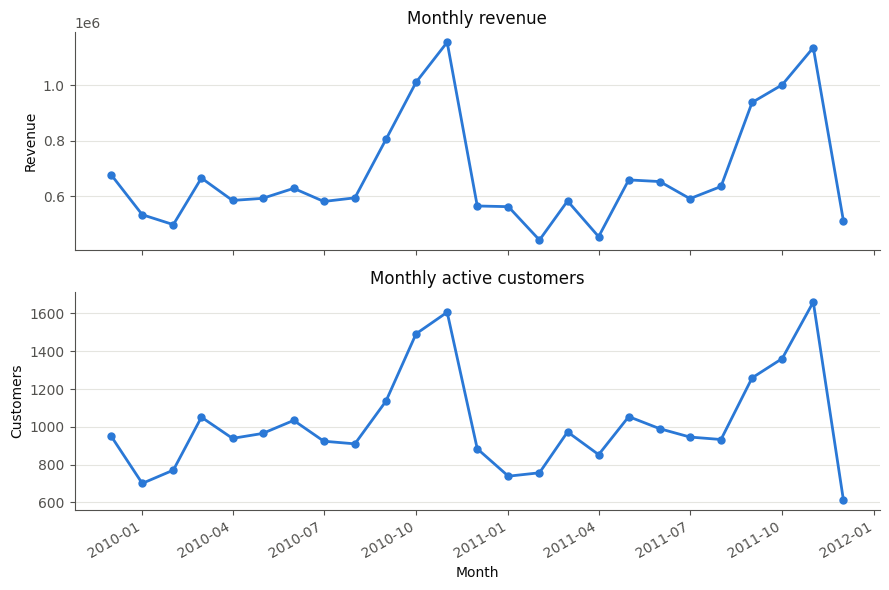
\includegraphics[width=0.85\textwidth]{figures/ch6_monthly_revenue_customers.png}
\end{center}

A typical full month has about \textbf{1,040 purchasing customers} (median 965) and \textbf{revenue of about GBP 690K} (median GBP 595K), ranging from GBP 442K (Feb 2011) to GBP 1.16M (Nov 2010). Both series are clearly \textbf{seasonal}: a steady climb from late summer to a peak in \textbf{October--November} (Nov 2010: GBP 1.16M; Nov 2011: GBP 1.14M; Oct 2010 and Oct 2011: GBP 1.0M each), driven by pre-Christmas ordering, followed by a sharp fall in December (Dec 2010: GBP 565K, 884 customers) through February. The first month (Dec 2009) and the last month (Dec 2011, only 9 days of data) are partial periods.

<<<<<<< HEAD
\section{New vs Existing Customers}
\label{sec:6-6}
=======
Two consequences carry into Chapter~\ref{ch:data-preparation}. Only about 1,040 of the 5,852 customers buy in a given month, so most customers purchase infrequently and churn must be judged over a window much longer than a month. And because behavior shifts with the season, the data must be split chronologically and results read per scoring week.
>>>>>>> 058c5219aa3dada1b3d09560b752a3e68791762b

\section{Existing Customers Drive Revenue}
\label{sec:4-4}

<<<<<<< HEAD
Monthly existing-customer counts grow steadily, from 281 (Dec 2009) to 1,501 (Nov 2011); monthly new-customer counts shrink from 951 in the first month (when every buyer is ``new'' by definition) to double digits by late 2011 (28 in Dec 2011). This is expected within a fixed two-year window: acquisition slows relative to the accumulated installed base.

\section{Revenue from New and Existing Customers}
\label{sec:6-7}

\begin{center}
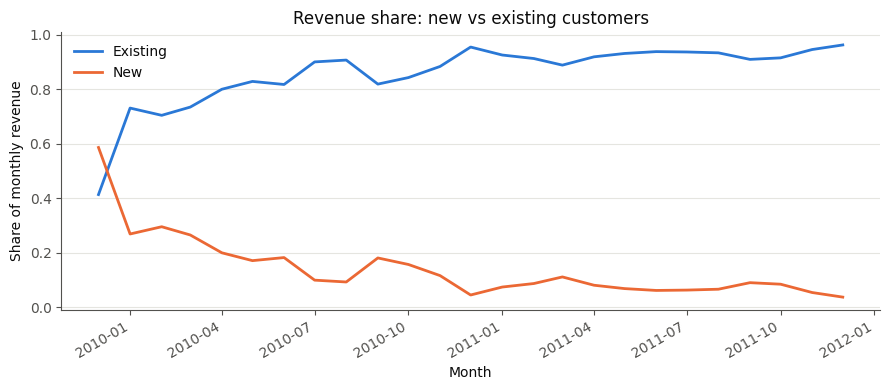
\includegraphics[width=0.85\textwidth]{figures/ch6_revenue_share_new_existing.png}
\end{center}

The existing-customer share of monthly revenue rises quickly from 41.4\% (Dec 2009, the only month where new customers can dominate, since every buyer is new in month one) to over 80\% by mid-2010, and stays in the 88--96\% range from late 2010 onward, ending at 96.2\% in Dec 2011. Over the full period, existing-customer occasions generate 14,687,090.56 (86.0\%) of occasion revenue versus 2,381,477.41 (14.0\%) from new-customer occasions -- directly supporting the business case (Chapter~\ref{ch:business-understanding}) for prioritizing retention of existing customers over new-customer acquisition.

\textbf{Note.} This is an \emph{occasion-level} split (each occasion is separately labeled new or existing). Section~\ref{sec:6-8} instead reports a \emph{customer-level} split (one-time vs.\ repeat, with all of a customer's revenue attributed to whichever group they belong to), which is why the ``new'' share here (14.0\%) differs from the ``one-time'' share there (3.3\%) -- the two percentages answer different questions and are not inconsistent.

\section{Repeat Customer Analysis}
\label{sec:6-8}
=======
Each customer's purchase occasions are ordered in time; the first occasion is \textbf{new}, every later one is \textbf{existing}. At the customer level, over the whole period:
>>>>>>> 058c5219aa3dada1b3d09560b752a3e68791762b

\begin{center}
\begin{tabular}{@{}p{3cm}p{2.3cm}p{2.3cm}p{2.6cm}p{2.3cm}@{}}
    \toprule
    Segment & Customers & Orders & Revenue (GBP) & Revenue share \\
    \midrule
    One-time & 1,618 (27.65\%) & 1,618 (4.42\%) & 555,999.97 & 3.26\% \\
    Repeat & 4,234 (72.35\%) & 34,976 (95.58\%) & 16,512,568.00 & 96.74\% \\
    \bottomrule
\end{tabular}
\end{center}

\textbf{Repeat customers} -- those with two or more purchase occasions -- are 72.3\% of the customer base but generate \textbf{95.6\% of orders and 96.7\% of revenue}. Almost all realized revenue already comes from customers who buy more than once, which is the direct business case (Chapter~\ref{ch:problem-approach}) for a retention strategy aimed at existing customers.

<<<<<<< HEAD
\section{Monthly Repurchase Analysis}
\label{sec:6-9}
=======
The same picture holds month by month. Each customer active in a month is counted once, as new in their first purchase month and existing in any later month:
>>>>>>> 058c5219aa3dada1b3d09560b752a3e68791762b

\begin{center}
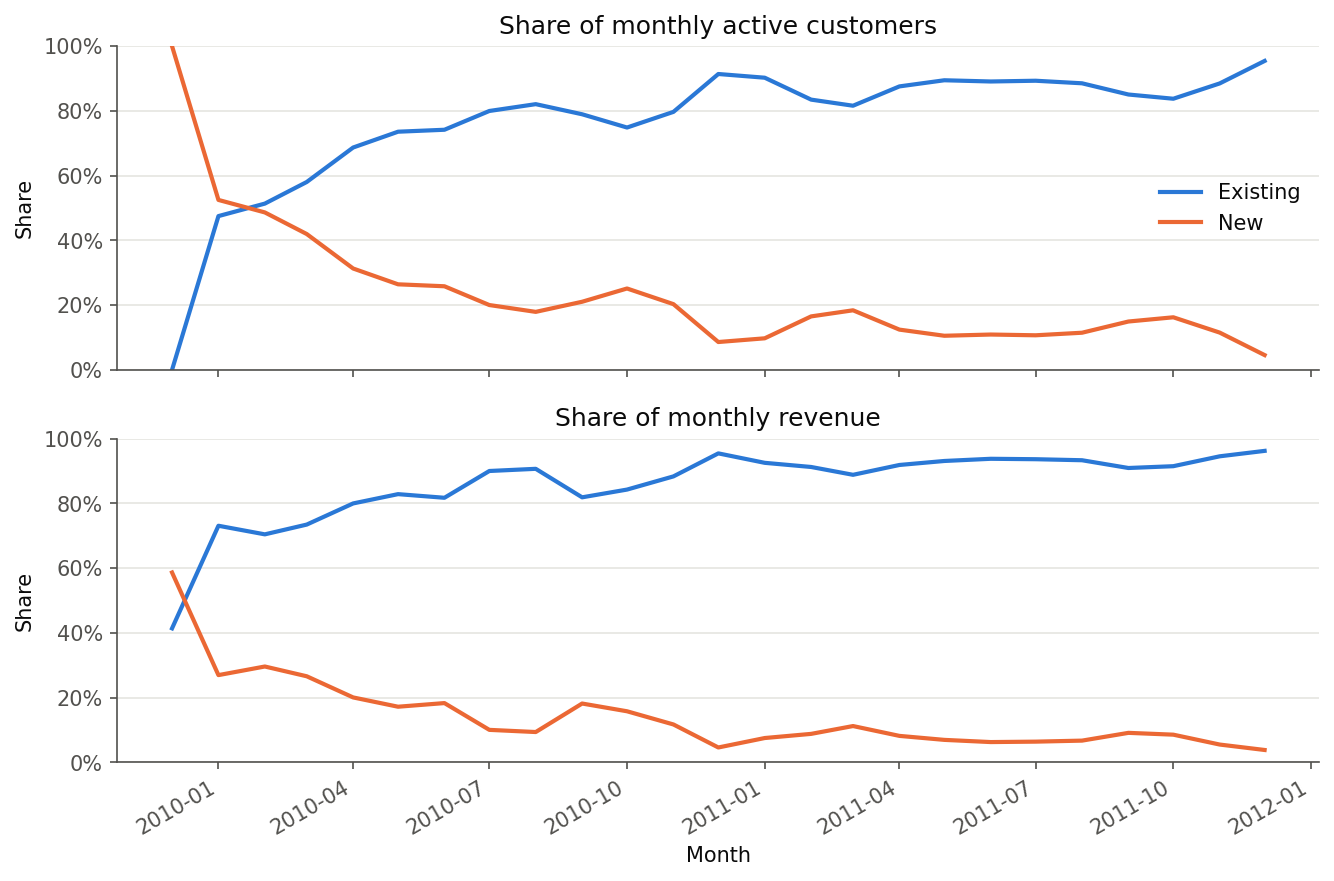
\includegraphics[width=0.85\textwidth]{figures/ch6_new_existing_share.png}
\end{center}

<<<<<<< HEAD
\section{Inter-Purchase Interval}
\label{sec:6-10}
=======
After the first months of data (Dec 2009 is 100\% new by construction), existing customers make up 80\% or more of monthly active customers from mid-2010 and 81.6--95.4\% throughout 2011, and their share of monthly revenue is higher still, in the 88--96\% range from late 2010 onward. Existing customers therefore dominate both who buys and how much is spent.

\section{Repurchase Interval and the 90-Day Horizon}
\label{sec:4-5}

Retail is a \textbf{non-contractual} setting: customers never cancel, so churn has to be inferred from a period without purchases. The gap between consecutive purchase occasions of the same customer tells how long that period should be. Note that the shares below are per \textbf{repurchase} (one gap per repeat occasion, 30,742 in total), not per customer: frequent buyers contribute more gaps, and one-time customers contribute none.
>>>>>>> 058c5219aa3dada1b3d09560b752a3e68791762b

\begin{center}
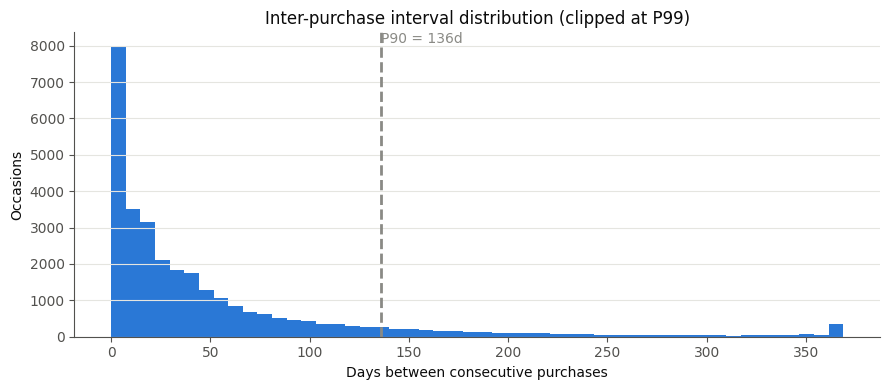
\includegraphics[width=0.85\textwidth]{figures/ch6_inter_purchase_interval.png}
\end{center}

\begin{center}
\begin{tabular}{@{}p{2.3cm}p{2.3cm}p{2.3cm}p{2.3cm}p{2.3cm}@{}}
    \toprule
    Mean & Std & Median & P90 & P99 \\
    \midrule
    52.1 d & 75.9 d & 25.0 d & 136.0 d & 368.9 d \\
    \bottomrule
\end{tabular}
\end{center}

<<<<<<< HEAD
Gaps between a customer's consecutive purchase occasions are highly right-skewed (mean 52.1 days vs.\ median 25.0 days; min 0.0 days, max 714.2 days). Two candidate values for \textbf{$R_{\max}$} are carried forward: \textbf{P90 $=$ 136.0 days} (adopted as the default activity threshold for the rest of this chapter) and P95 $=$ 207.0 days (used as a sensitivity check in Section~\ref{sec:6-15}).

\section{Customer Monetary and Behavioral Analysis}
\label{sec:6-11}
=======
Gaps are highly right-skewed (mean 52.1 days vs.\ median 25.0 days). \textbf{54.8\% of repurchases happen within 30 days} of the previous purchase -- the largest single group, but not yet representative of repurchasing as a whole. Extending the window to \textbf{90 days covers 82.8\% of repurchases}; beyond 150 days each 30-day bin holds under 2.5\% of gaps, and the open-ended 240+ bin collects the remaining 3.7\%.

\textbf{Choosing the horizon $H$.} The prediction horizon trades off three criteria:
>>>>>>> 058c5219aa3dada1b3d09560b752a3e68791762b

\begin{center}
\begin{tabular}{@{}p{1.6cm}p{5cm}p{4.6cm}@{}}
    \toprule
    $H$ (days) & Repurchases within $H$ & Training weeks after the embargoed split \\
    \midrule
    60 & 74.2\% & 37 \\
    \textbf{90} & \textbf{82.8\%} & \textbf{24} \\
    120 & 88.1\% & 10 \\
    \bottomrule
\end{tabular}
\end{center}

A shorter horizon labels as churned many customers who would in fact come back (noisier labels); a longer one detects churn later -- at odds with the goal of early identification (Section~\ref{sec:1-2}) -- and, on a two-year window, leaves far fewer labelable weeks for training once two $H$-day embargoes are subtracted (computed in Section~\ref{sec:5-9}). \textbf{$H = 90$ days} covers most repurchases while keeping 24 training weeks; moving to 120 days would add only 5 points of coverage at the cost of more than half the training weeks.

<<<<<<< HEAD
\section{Customer Lifecycle}
\label{sec:6-12}

Stages are illustrative, based on recency as of the last observed date and $R_{\max}$ (P90, from Section~\ref{sec:6-10}) -- not a final definition.
=======
The same distribution sets the \textbf{activity threshold} $R_{\max} = $ P90 $=$ 136 days: a customer whose last purchase is older than this is treated as already lapsed and is not scored. $H$ answers \emph{how long without a purchase counts as churn}; $R_{\max}$ answers \emph{who is still worth predicting for}.

\section{Customer Groups by Purchase Cadence}
\label{sec:4-6}

Customers are grouped by purchase cadence -- an illustrative grouping, not a final definition. \textbf{One-time} customers have only their first purchase (no gap yet); every other customer is grouped by their \textbf{average inter-purchase gap}, the mean of their own gaps from Section~\ref{sec:4-5}: 0--30, 30--90 or 90+ days. The average uses each customer's full history, which is fine for description; model features in Chapter~\ref{ch:data-preparation} only use history up to the snapshot date. For each group, AOV is the group's revenue divided by its purchase occasions.
>>>>>>> 058c5219aa3dada1b3d09560b752a3e68791762b

\begin{center}
\begin{tabular}{@{}p{3.2cm}p{2.3cm}p{2.6cm}p{2.3cm}p{2.3cm}@{}}
    \toprule
    Group & Customers & Customer share & AOV (GBP) & Revenue share \\
    \midrule
    One-time & 1,618 & 27.65\% & 343.63 & 3.26\% \\
    0--30 days & 755 & 12.90\% & 598.50 & 48.70\% \\
    30--90 days & 1,775 & 30.33\% & 385.56 & 33.45\% \\
    90+ days & 1,704 & 29.12\% & 396.65 & 14.59\% \\
    \bottomrule
\end{tabular}
\end{center}

Customers whose usual rhythm is under 90 days generate \textbf{82.2\% of revenue} (48.7\% + 33.5\%). Frequent buyers (under 30 days) are only 12.9\% of customers but 48.7\% of revenue, combining the most purchase occasions with the largest baskets (AOV 598.50 vs.\ 466.43 overall). The 90+ day group still buys, only slowly, and holds 14.6\% of revenue; one-time customers are over a quarter of the base yet only 3.3\% of revenue. The implication for the label: when a customer who normally returns within 90 days goes 90 days without a purchase, that is a departure from their usual rhythm -- exactly the signal a 90-day churn label captures, and it concerns the customers who carry most of the revenue.

\textbf{Per repurchase vs.\ per customer.} The 82.8\% of Section~\ref{sec:4-5} is a share of repurchases, dominated by frequent buyers. Per customer, only \textbf{59.8\% of repeat customers} have an average gap under 90 days (17.8\% under 30 days, 41.9\% at 30--90 days) and 40.2\% buy more slowly; adding the one-time customers, who have no repurchase at all, explains why the churn rate at $H = 90$ is close to one half (Section~\ref{sec:5-7}) even though most repurchases happen within 90 days.

\begin{center}
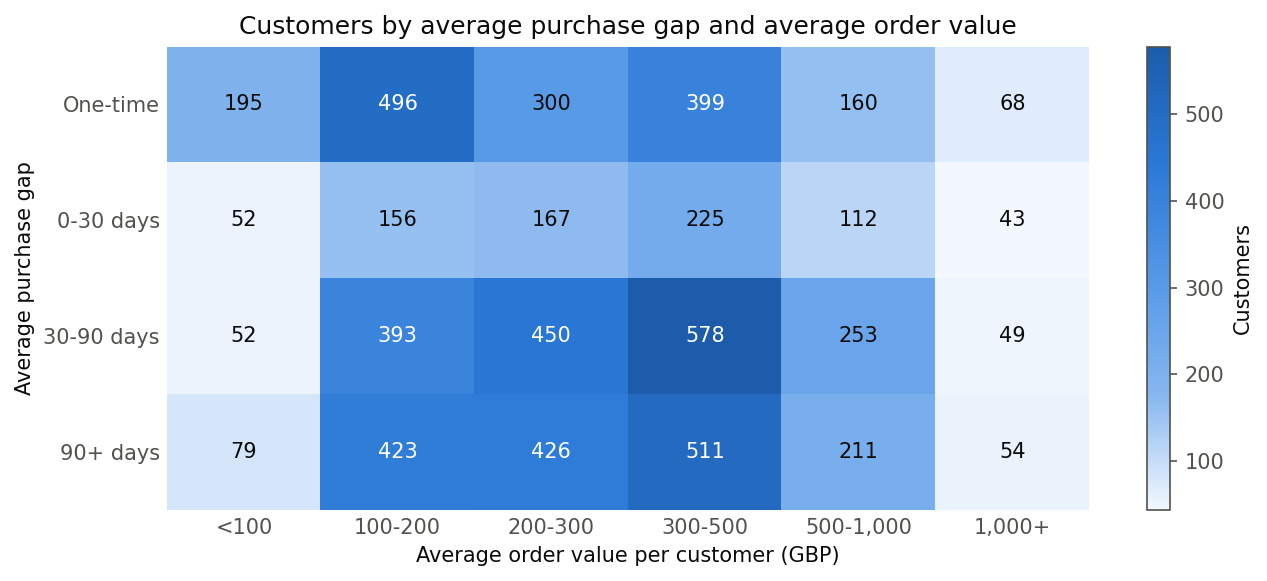
\includegraphics[width=0.85\textwidth]{figures/ch6_lifecycle_aov_heatmap.png}
\end{center}

Crossing the cadence groups with customer AOV shows that purchase cadence and basket size are largely independent: every repeat group peaks in the 300--500 GBP band (225, 578 and 511 customers), while one-time customers peak lower, at 100--200 GBP (496 customers). Large baskets (1,000+ GBP) are rare and spread evenly across all four groups (43--68 customers each) -- so frequency/recency and monetary behavior carry different information and both belong in the feature set.

\textbf{Cadence mix over time.} Regrouping every (customer, week) row into the same four groups, using the purchase history \emph{as of that week} (average gap so far $=$ (last purchase $-$ first purchase) $\div$ (purchases $- 1$)), tracks how the customer-base mix evolves:

\begin{center}
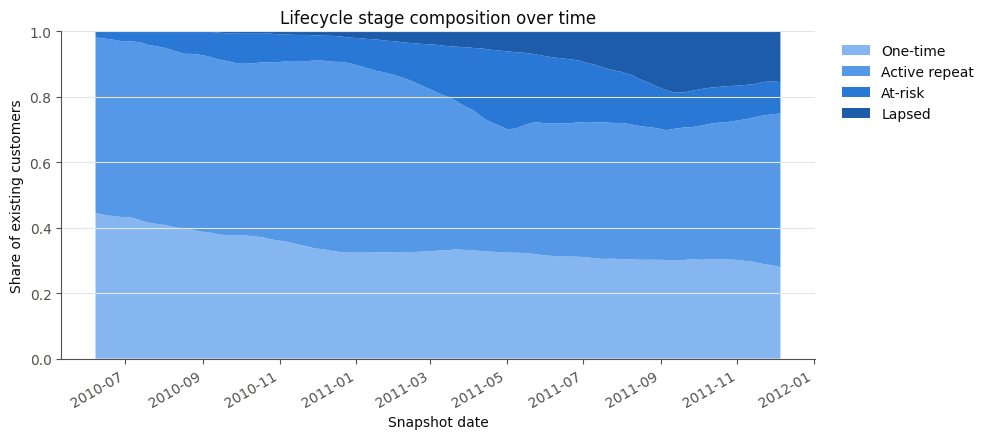
\includegraphics[width=0.85\textwidth]{figures/ch6_lifecycle_stage_trend.png}
\end{center}

Over the 79 weekly snapshots (Jun 2010 -- Dec 2011), the 90+ day share grows from 6.5\% to 29.0\% while the One-time share falls from 44.5\% to 28.0\%. Part of this is mechanical: in a fixed two-year window, long gaps only become observable as customers age, so the trend should not be read as a pure change in behavior. It does, however, show that a growing part of the customer base drifts into slow repurchasing.

<<<<<<< HEAD
\section{RFM Exploration}
\label{sec:6-13}
=======
\section{Key Findings and Design Decisions}
\label{sec:4-7}
>>>>>>> 058c5219aa3dada1b3d09560b752a3e68791762b

\begin{center}
\begin{tabular}{@{}p{7.2cm}p{7cm}@{}}
    \toprule
    Finding & Design decision (Chapter~\ref{ch:data-preparation}) \\
    \midrule
    776,577 valid rows (72.8\%) = 36,594 invoices of 5,852 customers, Dec 2009 -- Dec 2011 & Customer histories built from valid purchase occasions only (Sections~\ref{sec:5-1}--\ref{sec:5-3}) \\
    About 1,040 customers and GBP 690K revenue per month; peak in Oct--Nov, sharp drop in Dec & Chronological split with embargo; results read per scoring week (Section~\ref{sec:5-9}) \\
    Only about 1,040 of 5,852 customers buy in a given month & Weekly snapshots of all active customers, judged over a multi-month window (Sections~\ref{sec:5-4}--\ref{sec:5-5}) \\
    Repeat customers: 72.3\% of customers, 95.6\% of orders, 96.7\% of revenue & Population focused on existing customers (Section~\ref{sec:5-4}) \\
    54.8\% of repurchases within 30 days, 82.8\% within 90 days; P90 gap $=$ 136 days & Label horizon $H = 90$ days (Section~\ref{sec:5-7}); activity threshold $R_{\max} = 136$ days (Section~\ref{sec:5-4}) \\
    Customers with an average gap under 90 days hold 82.2\% of revenue & A 90-day churn label flags departures from the usual rhythm of the most valuable customers \\
    One-time customers: 27.6\% of customers, 3.3\% of revenue & Kept in the population but reported as a separate segment \\
    Purchase cadence and AOV are largely independent & Features cover both frequency/recency and monetary behavior (Section~\ref{sec:5-6}) \\
    \bottomrule
\end{tabular}
\end{center}
<<<<<<< HEAD

Grouping customers into frequency deciles and averaging recency and monetary value within each decile shows a clear monotonic relationship:

\begin{center}
\begin{tabular}{@{}p{3.2cm}p{3.2cm}p{3.2cm}@{}}
    \toprule
    Frequency decile & Mean recency (days) & Mean monetary (GBP) \\
    \midrule
    1 (lowest) & 335.1 & 409.8 \\
    5 & 212.2 & 1,070.2 \\
    10 (highest) & 35.1 & 16,670.9 \\
    \bottomrule
\end{tabular}
\end{center}

Customers who buy more often also buy more recently and spend far more per customer -- directly motivating RFM-style features for the churn model.

\section{Churn Exploration}
\label{sec:6-14}

Using provisional labels ($H = 90$ days, $R_{\max} =$ P90 $= 136.0$ days): of 208,751 weekly active snapshot rows, 172,550 are labelable (their full prediction window is observed before the data end). The provisional overall churn rate is \textbf{48.0\%} -- with many one-time buyers, churn is close to the \emph{majority} class here, not a rare event, which changes how PR-AUC and Precision should be read (Section~\ref{sec:3-14}/Chapter~\ref{ch:evaluation}).

\begin{center}
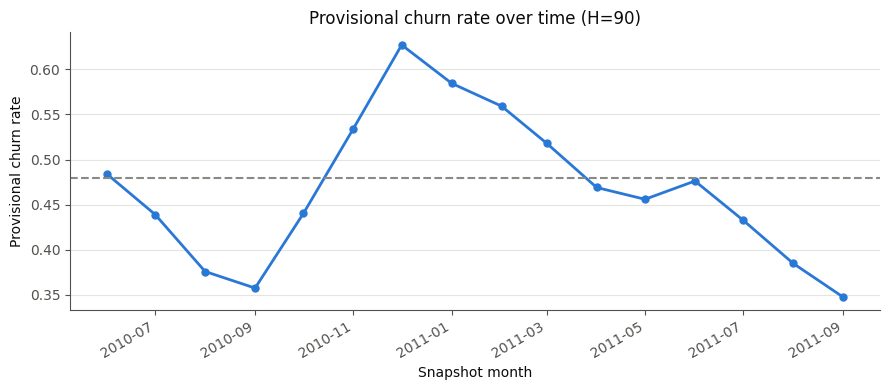
\includegraphics[width=0.85\textwidth]{figures/ch6_churn_rate_by_month.png}
\end{center}

The monthly churn rate ranges from 34.8\% (Sep 2011) to 62.7\% (Dec 2010), noticeably higher in the winter months (Dec--Feb) than the rest of the year.

Churn rate falls sharply and monotonically with both monetary and frequency decile:

\begin{center}
\begin{tabular}{@{}p{3cm}p{3.6cm}p{3.6cm}@{}}
    \toprule
    Decile & Churn rate (by monetary) & Churn rate (by frequency) \\
    \midrule
    1 (lowest) & 93.7\% & 100.0\% \\
    5 & 52.0\% & 53.9\% \\
    10 (highest) & 8.5\% & 3.2\% \\
    \bottomrule
\end{tabular}
\end{center}

This strong univariate separation is an encouraging sign for predictive feasibility and reinforces the case for RFM-style features.

\section{Snapshot Population and Design Feasibility}
\label{sec:6-15}

\textbf{1. Snapshot scheme comparison.}

\begin{center}
\begin{tabular}{@{}p{3.6cm}p{3cm}p{3.6cm}@{}}
    \toprule
    Scheme & Rows & Rows per customer \\
    \midrule
    Daily & 1,477,637 & 256.8 \\
    Weekly, all active & 208,751 & 36.5 \\
    Weekly, episode cooldown ($C=90$) & 20,151 & 3.5 \\
    \bottomrule
\end{tabular}
\end{center}

A daily grid carries 7.1$\times$ the rows of weekly-all, confirming the cost of daily snapshots. The episode-cooldown rule cuts weekly-all rows by more than 90\%, as intended, while class balance stays close across all three schemes (daily 48.0\%, weekly-all 48.0\%, weekly-episode 49.5\% churn) -- the subsampling does not materially bias the label distribution.

\textbf{2. Effect of $R_{\max}$ on population and churn rate.}

\begin{center}
\begin{tabular}{@{}p{2.6cm}p{2.6cm}p{2.9cm}p{2.9cm}p{2.3cm}@{}}
    \toprule
    $R_{\max}$ & Days & Active rows & Active customers & Churn rate \\
    \midrule
    P90 & 136.0 & 208,751 & 5,725 & 48.0\% \\
    P95 & 207.0 & 254,540 & 5,835 & 52.8\% \\
    \bottomrule
\end{tabular}
\end{center}

Loosening the activity threshold from P90 to P95 admits more marginal customers and pushes the observed churn rate up by nearly 5 points -- the final $R_{\max}$ choice will materially change the label distribution.

\textbf{3. Weekly Scoring Population.}

\begin{center}
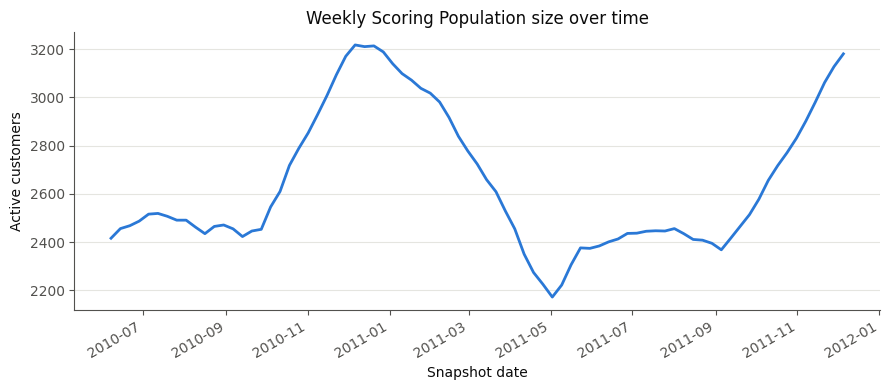
\includegraphics[width=0.85\textwidth]{figures/ch6_weekly_scoring_population.png}
\end{center}

The weekly Scoring Population -- the pool from which marketing selects Top-K each week -- is stable, averaging 2,642 active customers per week (range 2,172--3,218) over the 79 snapshot weeks. This is far larger than the 20,151-row, episode-restricted training population, confirming that the episode rule must not be applied to scoring.

\textbf{4. Feasibility check.} For each candidate $H$, counting labelable weekly scoring dates after warm-up and after the embargoes of Section~\ref{sec:7-9} (targeting 8 validation and 10 test weeks):

\begin{center}
\begin{tabular}{@{}p{1.8cm}p{2.6cm}p{2.3cm}p{2.1cm}p{2.1cm}@{}}
    \toprule
    $H$ & Labelable weeks & Train weeks & Val weeks & Test weeks \\
    \midrule
    60 & 71 & 37 & 8 & 10 \\
    90 & 66 & 24 & 8 & 10 \\
    120 & 62 & 10 & 8 & 10 \\
    \bottomrule
\end{tabular}
\end{center}

All three candidates clear the $\geq 8$ test-week bar, but $H = 120$ leaves only 10 training weeks, too thin to be practical, while $H = 60$'s shorter horizon is less useful operationally. \textbf{$H = 90$ (24 training weeks) is the best-supported choice}, matching the illustrative timeline already used in Section~\ref{sec:7-9}.

\section{Key Findings}
\label{sec:6-16}

\textbf{Revenue composition.} Repeat customers are 72.3\% of customers (4,234 of 5,852) but generate 96.7\% of revenue and 95.6\% of orders -- existing-customer retention is where almost all the revenue already is, which is the direct business case for this project.

\textbf{Heterogeneity.} Customer revenue is extremely right-skewed (mean 2,916.71 vs.\ median 856.02 GBP). The top 1\% of customers by revenue (``wholesale-like'') are only 1.0\% of customers but 32.1\% of revenue -- consistent with Online Retail II's known mix of UK retail and wholesale buyers (Section~\ref{sec:5-5}).

\textbf{Repeat purchasing.} The monthly repurchase rate among eligible existing customers averages 23.3\% (range 10.1\%--36.0\% across 24 months) -- noisier month to month than seasonal, unlike raw revenue, which clearly peaks in Nov 2010 and dips in Feb 2011.

\textbf{Purchase intervals $\rightarrow R_{\max}$.} Gaps between consecutive purchases are highly skewed: median 25 days, mean 52 days, P90 $=$ 136 days, P95 $=$ 207 days. These set the $R_{\max}$ candidates used throughout this chapter (136 / 207 days).

\textbf{Churn behavior.} At $H = 90$ days and $R_{\max} =$ P90, the provisional churn rate is \textbf{48.0\%} across 172,550 labelable active snapshot rows -- churn is close to a majority class here, not a rare event, exactly the scenario Section~\ref{sec:3-14}/Chapter~\ref{ch:evaluation} warn about for reading PR-AUC and Precision. Loosening the activity threshold to $R_{\max} =$ P95 admits more marginal customers and pushes the observed rate up to 52.8\%, so the final $R_{\max}$ choice will materially change the label distribution.

\textbf{Snapshot design feasibility.} Weekly-all active population is stable (mean $\approx$2,642 customers/week, range 2,172--3,218 over 79 weeks). The episode-cooldown rule ($C=90$) cuts training rows from 208,751 (weekly-all) to 20,151 -- a $>$90\% reduction, as intended. A daily grid would carry 1,477,637 rows ($\approx$7.1$\times$ weekly-all), confirming the cost of daily snapshots. For the embargoed split (8 validation / 10 test weeks, matching Section~\ref{sec:7-9}'s illustration): train weeks fall sharply as $H$ grows -- 37 ($H=60$), 24 ($H=90$), only 10 ($H=120$) -- because the $\approx$2-year span leaves little slack once two $H$-day embargoes are subtracted. All three candidates clear the $\geq 8$ test-week bar, but $H = 120$'s 10 training weeks is too thin to be practical; \textbf{$H = 90$ (24 train weeks) is the best-supported choice}, matching the illustrative timeline already used in Section~\ref{sec:7-9}.

\textbf{Data limitations.} 22.8\% of raw rows have no Customer ID (the single largest data-quality issue, ahead of duplicates at 3.2\%, invalid quantity/price at 2.4\%, cancellations at 1.8\%, and non-product codes at 0.6\%) and are necessarily excluded from any customer-level analysis. Combined, the valid-transaction rules keep 72.8\% of raw rows for analysis -- consistent with Section~\ref{sec:7-2}'s definition, applied here provisionally.
=======
>>>>>>> 058c5219aa3dada1b3d09560b752a3e68791762b


\chapter{Data Preparation}
\label{ch:data-preparation}
\section{Objective}
\label{sec:5-1}

Turn the cleaned transactions into a leakage-safe modeling dataset of \textbf{Customer $\times$ Snapshot Date} rows: clean the raw rows (Section~\ref{sec:5-2}), build the weekly populations (Section~\ref{sec:5-3}), attach the churn label (Section~\ref{sec:5-4}) and point-in-time features (Section~\ref{sec:5-5}), then split the rows chronologically with an embargo (Section~\ref{sec:5-6}). The chapter implements the design decisions of Section~\ref{sec:4-7} with one frozen configuration:

\begin{center}
\begin{tabular}{@{}p{5.2cm}p{2.6cm}p{6.3cm}@{}}
    \toprule
    Parameter & Value & Origin \\
    \midrule
    Prediction horizon $H$ & 90 days & Repurchase coverage and training-data trade-off (Section~\ref{sec:4-5}) \\
    Activity threshold $R_{\max}$ & 136 days & P90 of the inter-purchase gap (Section~\ref{sec:4-5}) \\
    Episode cooldown $C$ & 90 days ($= H$) & Non-overlapping label windows for training \\
    Warm-up & 6 months & Minimum history before the first snapshot \\
    Snapshot frequency & Weekly (Mondays) & Matches a weekly Top-K marketing cycle \\
    \bottomrule
\end{tabular}
\end{center}

\section{Data Cleaning}
\label{sec:5-2}

The raw-value conventions -- cancellation invoices, non-product stock codes and missing Customer ID -- are described in Section~\ref{sec:3-5}. Here they become one reproducible \textbf{valid purchase} filter. A row is kept only if it:
\begin{itemize}
    \item has a Customer ID (otherwise it cannot be attached to any customer history);
    \item is not a cancellation (invoice starting with ``C''); cancellations are kept separately for the cancellation features of Section~\ref{sec:5-5};
    \item has Quantity $> 0$ and Price $> 0$;
    \item is a real product, not a non-product stock code;
    \item is not an exact duplicate of an earlier row.
\end{itemize}
Non-product stock codes are discovered empirically -- codes that do not start with a digit, unlike normal product codes such as \texttt{85048} or \texttt{79323P} -- rather than assumed in advance. Each issue is first measured on the full raw dataset (rows may overlap across rules):

\begin{center}
\begin{tabular}{@{}p{6cm}p{3.5cm}p{3.5cm}@{}}
    \toprule
    Issue & Rows & Share of rows \\
    \midrule
    Missing Customer ID & 243,007 & 22.77\% \\
    Exact duplicates & 34,335 & 3.22\% \\
    Invalid Quantity or Price ($\leq 0$) & 25,700 & 2.41\% \\
    Cancellations (Invoice starts with ``C'') & 19,494 & 1.83\% \\
    Non-product stock codes & 6,093 & 0.57\% \\
    \bottomrule
\end{tabular}
\end{center}

\textbf{Result.} Missing Customer ID is by far the largest issue. Combining all rules keeps \textbf{776,577 of 1,067,371 rows (72.8\%)} and 5,852 of the original 5,942 customers; the remaining 90 customers' entire history consists of invalid rows. The valid rows are then collapsed into \textbf{purchase occasions}, one per distinct invoice, carrying the invoice's earliest timestamp, summed revenue and quantity, and the set of products bought. This yields \textbf{36,594 purchase occasions across 5,852 customers}. Frequency, inter-purchase gaps and the churn label are all computed on occasions, not rows.

\section{Population Construction}
\label{sec:5-3}

\textbf{Time window.} Customer histories span the full data period, \textbf{2009-12-01 to 2011-12-09}. The first 6 months are a warm-up, so that every customer has some history at the first snapshot; snapshots are then taken every Monday from \textbf{2010-06-07 to 2011-12-05}, giving \textbf{79 weekly snapshot dates}.

\textbf{Eligibility.} At each snapshot date $t$, a customer is \textbf{eligible (active)} if:
\begin{enumerate}
    \item at least one valid purchase exists on or before $t$ (existing customer);
    \item Recency at $t$ $\leq R_{\max} = 136$ days (still active, not already lost).
\end{enumerate}
Customers beyond $R_{\max}$ leave the base and re-enter if they purchase again. The eligible rows of all 79 weeks form \textbf{one weekly active-customer base table}. Features and labels are computed once on this table, and the two populations are flags on it, which guarantees both use identical feature and label definitions:

\begin{center}
\begin{tabular}{@{}p{4.6cm}p{9.5cm}@{}}
    \toprule
    Flag & Rule \\
    \midrule
    \texttt{in\_scoring\_population} & Row is active and the customer is not under suppression at $t$. The historical data contain no real campaigns, so suppression is empty and every active row is in the \textbf{Scoring Population} (see Section~\ref{sec:7-1}). Used for validation, test and weekly scoring. \\
    \texttt{in\_training\_sample} & Row selected by the eligibility-episode rule below; the \textbf{Training Population}. \\
    \texttt{sample\_weight} & $1 /$ (number of weekly active rows of the customer in the training period); filled in once the training period is known (Section~\ref{sec:5-6}) and used only by the ablation scheme (Section~\ref{sec:6-10}). \\
    \bottomrule
\end{tabular}
\end{center}

\textbf{Training sample: the eligibility-episode rule.} Consecutive weekly snapshots of the same customer differ only slightly (mostly recency grows by 7 days) and their 90-day label windows overlap, so their labels are strongly correlated; long-history customers would also dominate training. The Training Population is therefore sampled per customer, in date order:
\begin{itemize}
    \item a training row is taken at the first weekly date $t$ at which the customer is active;
    \item the customer then contributes no further training row for a cooldown of $C = H = 90$ days -- the next one is the first weekly date $\geq t + C$ at which they are still active;
    \item a customer who exceeds $R_{\max}$ leaves the active base and, if they purchase again, starts a new episode.
\end{itemize}
Each customer's training labels then have non-overlapping prediction windows, and every customer contributes a similar number of rows. The rule is applied \textbf{only to training}; validation, test and scoring keep every active row. As an alternative scheme, all active rows can be used with the per-customer weight $1/n_i$ (\texttt{sample\_weight}), compared in Section~\ref{sec:6-10}.

\textbf{Result.} The base table has \textbf{208,764 weekly active rows of 5,725 customers}. A direct check confirms every \texttt{in\_training\_sample} row is also an \texttt{in\_scoring\_population} row -- the episode rule only subsets the active base, never adds to it:

\begin{center}
\begin{tabular}{@{}p{6.4cm}p{2.4cm}p{2.4cm}p{2.8cm}@{}}
    \toprule
    Population & Rows & Customers & Rows per customer \\
    \midrule
    Weekly, all active (Scoring Population) & 208,764 & 5,725 & 36.5 \\
    Weekly, episode cooldown ($C = 90$) (Training Population) & 20,152 & 5,725 & 3.5 \\
    \bottomrule
\end{tabular}
\end{center}

The episode rule cuts the weekly rows by more than 90\% for training (from 36.5 to 3.5 rows per customer) while keeping every customer.

\begin{center}
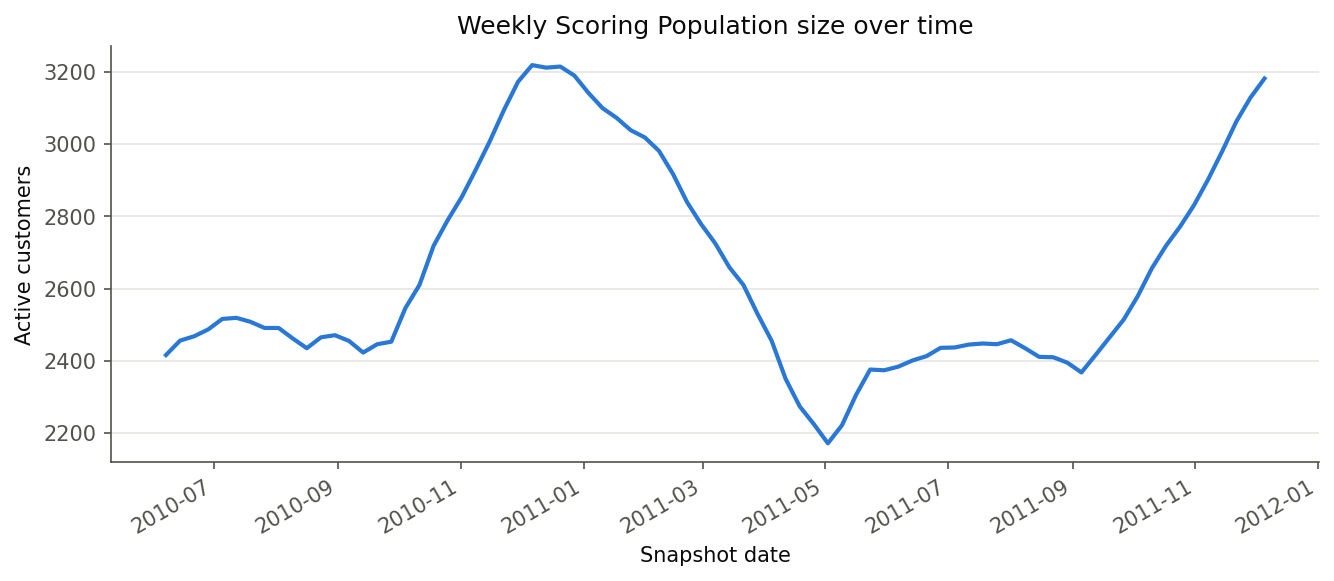
\includegraphics[width=0.85\textwidth]{figures/ch7_weekly_scoring_population.png}
\end{center}

The weekly Scoring Population -- the pool from which marketing would select its Top-K each week -- averages 2,643 active customers per week (range 2,172--3,218). It has no growth trend: year over year it stays flat, but within the year it is strongly seasonal, building up before Christmas and draining from January to May as customers pass the 136-day threshold.

\textbf{Sensitivity to $R_{\max}$.} The threshold decides who is labeled and scored. Loosening it from P90 to P95 admits more marginal customers and pushes the churn rate (label defined in Section~\ref{sec:5-4}) up by nearly 5 points, so the choice materially changes the label distribution:

\begin{center}
\begin{tabular}{@{}p{2.6cm}p{2.2cm}p{2.9cm}p{3.2cm}p{2.3cm}@{}}
    \toprule
    $R_{\max}$ & Days & Active rows & Active customers & Churn rate \\
    \midrule
    P90 (chosen) & 136.0 & 208,764 & 5,725 & 48.0\% \\
    P95 & 207.0 & 254,538 & 5,835 & 52.8\% \\
    \bottomrule
\end{tabular}
\end{center}

\section{Churn Label Construction}
\label{sec:5-4}

\textbf{Definition.} A row at snapshot date $t$ is labeled \textbf{churn $= 1$} if the customer makes no valid purchase in the prediction window $(t,\, t+H]$, and churn $= 0$ otherwise. Only the prediction window is used to determine churn, applying the same valid-purchase definition as Section~\ref{sec:5-2}. A row is \textbf{labelable} only if its full window is observed, i.e.\ $t + H \leq$ data end (2011-12-09); the last 13 weekly snapshots (2011-09-12 to 2011-12-05) can be scored but not labeled.

\textbf{Result.} At $H = 90$ days, \textbf{172,561 of the 208,764 base rows (82.7\%) are labelable}, and the churn rate on those rows is \textbf{48.0\%}. Churn is therefore close to a majority class here, not a rare event, which changes how PR-AUC and Precision should be read (Chapter~\ref{ch:evaluation}). It is close to one half even though 82.8\% of repurchases happen within 90 days, because that share is dominated by frequent buyers: per customer, 40\% of repeat customers buy more slowly than every 90 days and one-time customers have no repurchase at all (Section~\ref{sec:4-6}).

\textbf{Label EDA.} The episode-sampled training rows have a churn rate of 49.5\%, close to the 48.0\% of the full Scoring Population -- the subsampling does not materially bias the label distribution.

\begin{center}
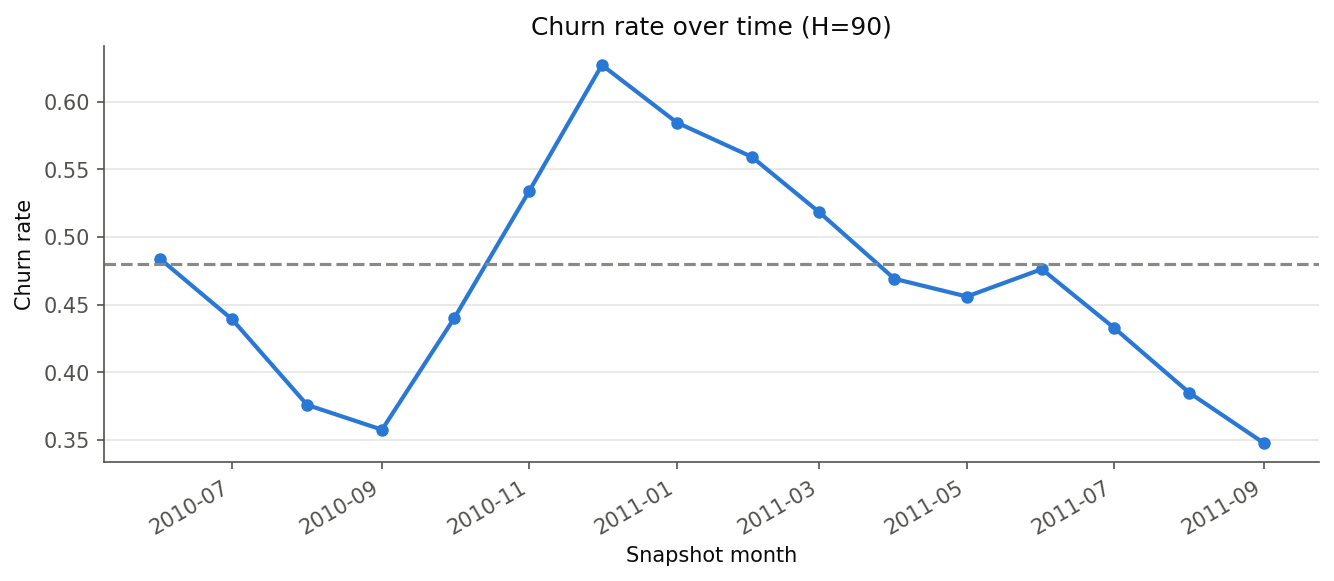
\includegraphics[width=0.85\textwidth]{figures/ch7_churn_rate_by_month.png}
\end{center}

The monthly churn rate ranges from 34.8\% (Sep 2011) to 62.7\% (Dec 2010) and is noticeably higher for snapshots taken in winter (Nov--Feb), whose 90-day windows fall in the post-Christmas low season -- the seasonality of Section~\ref{sec:4-3} carried into the label.

\section{Feature Engineering}
\label{sec:5-5}

Generate historical features using information available up to the snapshot date only, via a single backward as-of-merge primitive applied to cumulative per-occasion statistics -- the same mechanism used for recency itself, so every feature is leakage-safe by construction (verified explicitly in Section~\ref{sec:5-6}). A representative subset of each standard churn-feature group is implemented: RFM (recency, frequency, monetary), purchase behavior (average order value), temporal behavior (tenure, mean inter-purchase gap, recency relative to that gap, activity in the last 90 days), product behavior (distinct products so far) and cancellation behavior (cancellation count and value share so far).

\begin{center}
\begin{tabular}{@{}p{3.6cm}p{2.3cm}p{2.3cm}p{3.2cm}@{}}
    \toprule
    Feature & Mean & Median & Max \\
    \midrule
    Recency (days) & 50.5 & 41.6 & 136.0 \\
    Frequency so far & 6.56 & 4 & 367 \\
    Monetary so far (GBP) & 3,152.65 & 1,105.74 & 569,501.50 \\
    Avg.\ order value so far (GBP) & 393.39 & 302.53 & 25,784.32 \\
    Tenure (days) & 277.9 & 248.8 & 733.9 \\
    Mean inter-purchase gap so far (days) & 76.9 & 56.0 & 714.2 \\
    Recency / typical gap & 300.0 & 0.63 & 195,604 \\
    Activity in last 90 days (occasions) & 4.17 & 1 & 361 \\
    Distinct products so far & 86.2 & 53 & 2,515 \\
    Cancellations so far & 1.49 & 0 & 112 \\
    Cancellation value share so far & 0.022 & 0.000 & 0.896 \\
    \bottomrule
\end{tabular}
\end{center}

\textbf{A known instability.} \texttt{recency / typical gap} is undefined for the 43,970 rows where the customer has only one occasion so far (no prior gap exists) and is set to \texttt{NaN}. A further 31 rows had a \texttt{mean\_gap\_so\_far} of exactly zero (customers with multiple invoices at the same instant), which would otherwise divide to \texttt{inf} and break downstream modeling in Chapter~\ref{ch:modeling} -- these are also set to \texttt{NaN} rather than \texttt{inf}. Even after this fix the ratio's long tail is extreme (max 195,604, against a median of 0.63) because it divides by a very small but non-zero typical gap; a stricter pipeline would additionally winsorize this feature before modeling.

\textbf{Feature distributions.} The figure below shows each feature on the 172,561 labeled rows, split by churn outcome (shares of each class's rows; right-skewed and count features on a symmetric-log axis, cut at their 99th percentile):

\begin{center}
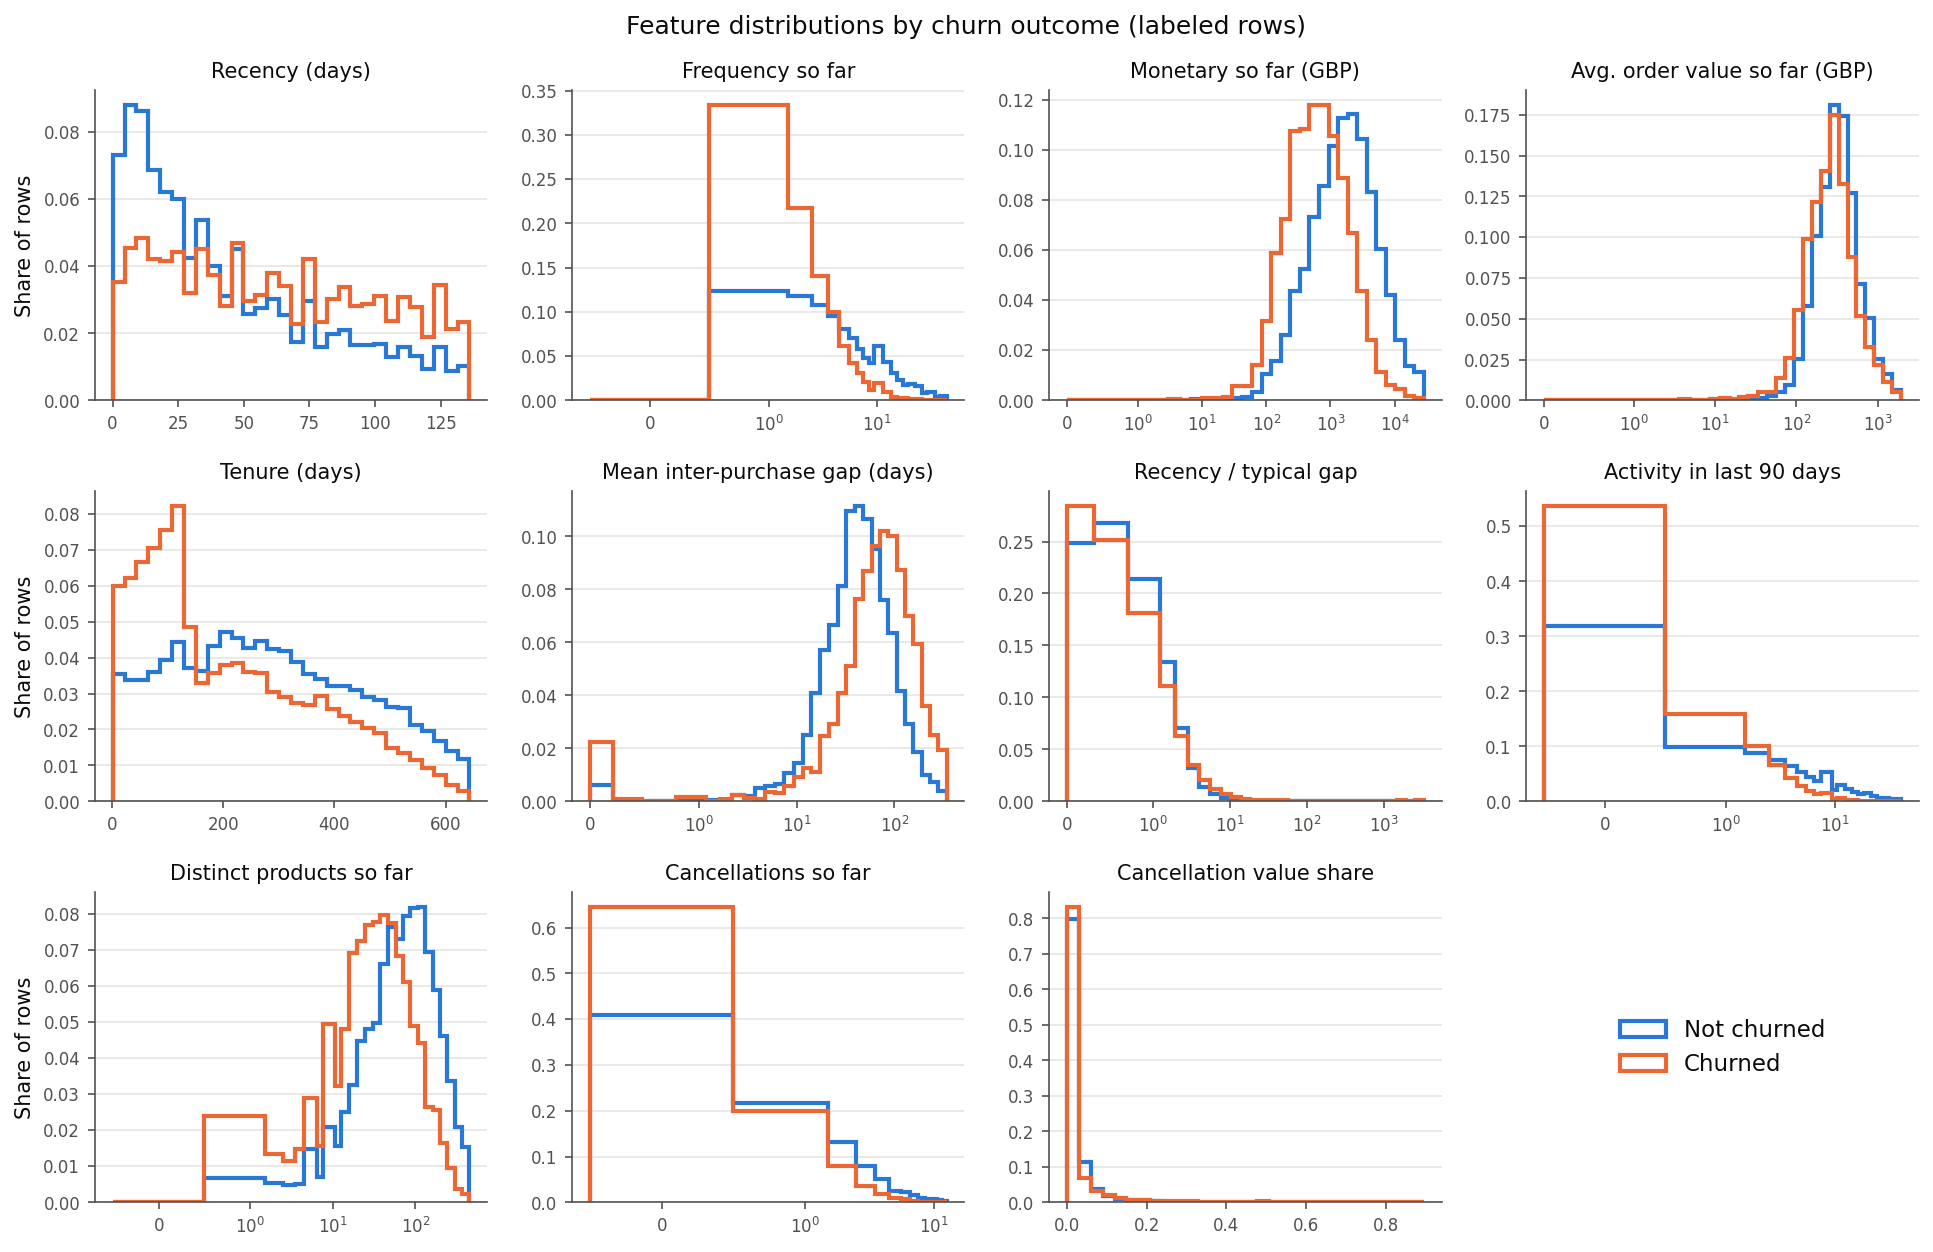
\includegraphics[width=\textwidth]{figures/ch7_feature_distributions.png}
\end{center}

\begin{itemize}
    \item \textbf{Strong separation} for the RFM and activity features. Non-churned rows cluster at low recency (median 33 days), while churned rows spread almost evenly up to 136 days (median 57). A third of churned rows have a single purchase so far, against 12\% of non-churned rows (median frequency 2 vs.\ 5), and their median monetary value is \pounds616 vs.\ \pounds1,688. 54\% of churned rows had no purchase in the last 90 days, against 32\%.
    \item \textbf{Moderate separation} for tenure (median 173 vs.\ 270 days), the mean inter-purchase gap (74 vs.\ 44 days) and distinct products (34 vs.\ 71): churners tend to be newer, slower and narrower buyers.
    \item \textbf{Weak separation} for average order value (median \pounds269 vs.\ \pounds324) and recency relative to the typical gap, whose two distributions nearly overlap. Rows with cancellations churn \emph{less} (65\% of churned rows have none, against 41\%), because cancellations come with more buying overall.
    \item \textbf{Skew and missing values.} Monetary, frequency and product counts span several orders of magnitude, which motivates the log transform applied before modeling (Chapter~\ref{ch:modeling}); the two gap features are missing for 22.5\% of labeled rows (one-time customers), handled by a median imputer fitted on training rows only.
\end{itemize}

\textbf{Churn by feature decile.} Churn also falls steadily with point-in-time purchase behavior:

\begin{center}
\begin{tabular}{@{}p{3cm}p{4.2cm}p{4.2cm}@{}}
    \toprule
    Decile & Churn rate (by frequency so far) & Churn rate (by monetary so far) \\
    \midrule
    1 (lowest) & 64.1\% & 75.5\% \\
    5 & 56.2\% & 54.5\% \\
    10 (highest) & 9.0\% & 12.7\% \\
    \bottomrule
\end{tabular}
\end{center}

The top deciles churn far less than the bottom ones -- a clear univariate signal for frequency and monetary features. The frequency curve is not monotonic in its lower deciles because many rows tie at one or two purchases so far. These point-in-time gaps are narrower than an end-of-data view would suggest, since that view would let customers' future purchases inflate their frequency and monetary values.

\section{Leakage Prevention and Temporal Split}
\label{sec:5-6}

\textbf{Leakage prevention.} No future information may be used in feature construction; the prediction window is reserved for label construction. A direct check re-derives one feature (\texttt{frequency\_so\_far}) for every base row and asserts its source timestamp never exceeds the row's snapshot date; this passes for all 208,764 rows, confirming the as-of-merge construction is leakage-safe by result, not only by design. Aggregates that depend on the whole dataset (scalers, encoders, imputation values, percentile thresholds) are fitted on the training period only, once modeling starts in Chapter~\ref{ch:modeling}.

\textbf{Caveat.} $R_{\max}$ and $H$ themselves were chosen from inter-purchase gaps measured over the \emph{full} dataset in Chapter~\ref{ch:data-understanding}, not the training period alone. A stricter pipeline would re-derive these thresholds from training-period data only; here they are treated as fixed configuration, consistent with their role as project-level design choices rather than learned parameters.

\textbf{Temporal split with embargo.} Split chronologically by snapshot date into train, validation and test, with an \textbf{embargo of $H$ days} between consecutive periods:
\begin{align*}
    \text{first validation date} &\geq \text{last training date} + H \\
    \text{first test date} &\geq \text{last validation date} + H
\end{align*}
Without the embargo, labels of late training snapshots are observed during the validation period, so the model effectively learns from a period it is later evaluated on.

\begin{center}
\begin{tabular}{@{}p{2.6cm}p{6.4cm}p{5cm}@{}}
    \toprule
    Split & Rows used & Purpose \\
    \midrule
    Train & \texttt{in\_training\_sample} rows in the train period & Fit candidate models \\
    Validation & \texttt{in\_scoring\_population} rows in the validation period & Tuning, model selection, calibration fit \\
    Final refit & \texttt{in\_training\_sample} rows re-derived over train + validation & Fit the selected model \\
    Test & \texttt{in\_scoring\_population} rows in the test period & Final, operation-like evaluation \\
    \bottomrule
\end{tabular}
\end{center}

Validation and test therefore measure performance exactly as the model would be used: ranking all active customers each week.

\textbf{Computed timeline ($H = 90$ days, weekly Mondays, 6-month warm-up).} Validation and test are sized to fixed operational targets (8 and 10 weeks) and taken from the end of the 66 labelable weekly dates working backward, with an embargo before each; train absorbs the remaining weeks:

\begin{center}
\begin{tabular}{@{}p{2.6cm}p{5.5cm}p{3cm}@{}}
    \toprule
    Period & Snapshot dates & Weekly dates \\
    \midrule
    Train & 2010-06-07 $\rightarrow$ 2010-11-15 & 24 \\
    \emph{Embargo} & \emph{90 days} & \emph{--} \\
    Validation & 2011-02-14 $\rightarrow$ 2011-04-04 & 8 \\
    \emph{Embargo} & \emph{90 days} & \emph{--} \\
    Test & 2011-07-04 $\rightarrow$ 2011-09-05 & 10 \\
    \bottomrule
\end{tabular}
\end{center}

\begin{center}
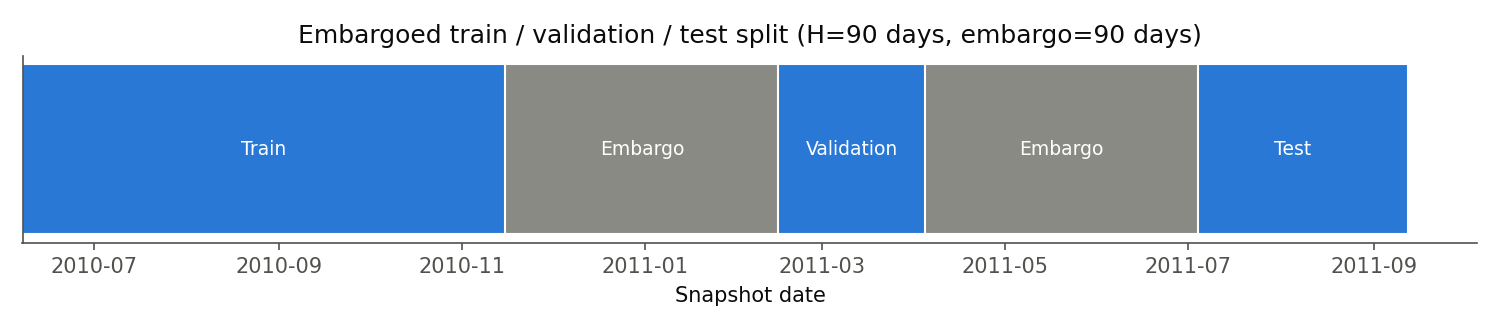
\includegraphics[width=0.85\textwidth]{figures/ch7_split_timeline.png}
\end{center}

24 of the 66 labelable weekly dates are consumed by the two embargoes; the remaining 42 weeks split into train/validation/test as above. The resulting churn rate differs by split -- a reminder that the seasonality already seen in Sections~\ref{sec:4-3} and~\ref{sec:5-4} shifts the base rate between periods, not just between individual weeks:

\begin{center}
\begin{tabular}{@{}p{2.6cm}p{2.3cm}p{2.6cm}p{2.3cm}@{}}
    \toprule
    Split & Active rows & Customers & Churn rate \\
    \midrule
    Train & 61,415 & 3,905 & 43.0\% \\
    Validation & 21,514 & 3,328 & 52.9\% \\
    Test & 24,252 & 2,907 & 40.1\% \\
    \bottomrule
\end{tabular}
\end{center}

\texttt{sample\_weight} is now computed for the 61,415 train-period active rows as $1 /$ (that customer's row count within the train period): it ranges from 0.0417 (a customer active in all 24 train weeks) to 1.0 (a customer active in only one), with a mean of 0.0636 -- confirming the weighting scheme gives every customer roughly equal total weight regardless of how many weekly rows they contributed, as intended for the ablation comparison in Section~\ref{sec:6-10}.

\textbf{Rows used per split.} The table above counts all active rows. Training fits only on the episode-sampled rows of the train period, while validation and test keep every active row -- because that is how the model is used, ranking all active customers each week:

\begin{center}
\begin{tabular}{@{}p{3.4cm}p{2.6cm}p{4.2cm}p{2.3cm}@{}}
    \toprule
    Split & Active rows & Rows used & Churn rate (rows used) \\
    \midrule
    Train & 61,415 & 6,453 episode rows (3,905 customers) & 46.7\% \\
    Validation & 21,514 & 21,514 (all active) & 52.9\% \\
    Test & 24,252 & 24,252 (all active) & 40.1\% \\
    Final refit (train start -- validation end) & -- & 12,019 episode rows (4,571 customers) & 51.3\% \\
    \bottomrule
\end{tabular}
\end{center}

For the final model, the episode rule is re-applied over the whole window from the first training date to the last validation date (Section~\ref{sec:6-7}); because the cooldown restarts over a longer window, the refit sample is nearly twice the size of the original training sample.

\textbf{Feasibility of $H$.} Applying the same allocation (8 validation and 10 test weeks, embargo of $H$ days before each) to each candidate horizon's labelable weekly dates:

\begin{center}
\begin{tabular}{@{}p{1.8cm}p{2.6cm}p{2.3cm}p{2.1cm}p{2.1cm}@{}}
    \toprule
    $H$ & Labelable weeks & Train weeks & Val weeks & Test weeks \\
    \midrule
    60 & 71 & 37 & 8 & 10 \\
    \textbf{90} & \textbf{66} & \textbf{24} & \textbf{8} & \textbf{10} \\
    120 & 62 & 10 & 8 & 10 \\
    \bottomrule
\end{tabular}
\end{center}

A longer horizon both removes labelable weeks at the end of the data and lengthens the two embargoes. All three candidates keep the 8 validation and 10 test weeks, but $H = 120$ leaves only 10 training weeks -- too thin to be practical -- which, together with the repurchase coverage of Section~\ref{sec:4-5}, supports $H = 90$.

\section{Conclusion}
\label{sec:5-7}

The final modeling table has one row per \textbf{Customer $\times$ Snapshot Date}, with the customer ID, snapshot date, a segment flag (one-time / repeat, based on frequency so far), the population flags (\texttt{in\_training\_sample}, \texttt{in\_scoring\_population}), the sample weight, the 11 historical features, the churn label and the split assignment -- produced by reproducible transformations from a single configuration. It has \textbf{208,764 rows and 20 columns}: 164,794 rows (79.0\%) are \texttt{repeat}-segment and 43,970 (21.0\%) are \texttt{one-time}-segment at their respective snapshot dates. The table is saved to \texttt{data/processed/}\allowbreak\texttt{modeling\_dataset\_h90.parquet} ($\approx$6.5\,MB) for direct reuse in Chapter~\ref{ch:modeling}.

\begin{center}
\begin{tabular}{@{}p{3.4cm}p{10.7cm}@{}}
    \toprule
    Step & Result \\
    \midrule
    Cleaning & 776,577 of 1,067,371 rows valid (72.8\%) $\rightarrow$ 36,594 purchase occasions of 5,852 customers \\
    Population & 208,764 weekly active rows of 5,725 customers over 79 weeks; 20,152 episode rows flagged for training \\
    Label & 172,561 labelable rows (82.7\%), churn rate 48.0\% -- close to balanced and seasonal \\
    Features & 11 point-in-time features in five groups; RFM and activity separate churners most clearly \\
    Split & Train 6,453 episode rows (46.7\% churn); validation 21,514 rows (52.9\%); test 24,252 rows (40.1\%); final refit 12,019 episode rows \\
    \bottomrule
\end{tabular}
\end{center}

Every row's features use only information up to its snapshot date, and the embargoed split keeps each evaluation period unseen by the periods before it -- so the models of Chapter~\ref{ch:modeling} are trained and evaluated as they would be used: scoring all active customers each week.


\chapter{Modeling}
\label{ch:modeling}
\section{Modeling Objective}
\label{sec:8-1}

Estimate $P(\text{Churn} = 1 \mid \text{Customer History at Snapshot})$ on the final modeling dataset built in Chapter~\ref{ch:data-preparation} (\texttt{modeling\_dataset\_h90.parquet}). Per the Section~\ref{sec:7-9} split table, \textbf{Train} is \texttt{in\_training\_sample} rows within \texttt{split=="train"} (6,453 rows, 46.7\% churn); \textbf{Validation} is every row in \texttt{split=="validation"} (21,514 rows, 52.9\% churn); \textbf{Test} is every row in \texttt{split=="test"} (24,252 rows, 40.1\% churn). The three periods have noticeably different churn base rates -- a direct consequence of the seasonality already documented in Section~\ref{sec:6-14}.

\textbf{Preprocessing (identical for every model in this chapter).} The nine right-skewed features (frequency, monetary value, average order value, tenure, mean gap, recency-to-gap ratio, recent activity, distinct products, cancellation count) are transformed with $\log(1+x)$, which has no fitted parameters and therefore cannot leak. Missing values (the two gap-based features for one-time customers) are filled with the training median, and all features are standardized; the imputer and scaler are fitted on the training rows only (Section~\ref{sec:7-8}).

\section{Baselines}
\label{sec:8-2}

\begin{center}
\begin{tabular}{@{}p{4.2cm}p{9.9cm}@{}}
    \toprule
    Baseline & Role \\
    \midrule
    Random ranking & Reference for Lift $= 1$ and PR-AUC $=$ churn rate. \\
    Recency rule & Rank customers by recency (longest since last purchase first). A strong, business-realistic rule the models must beat. \\
    \bottomrule
\end{tabular}
\end{center}

\begin{center}
\begin{tabular}{@{}p{3.2cm}p{1.8cm}p{1.8cm}p{2.4cm}p{1.8cm}@{}}
    \toprule
    Baseline & ROC-AUC & PR-AUC & Precision@10\% & Lift@10\% \\
    \midrule
    Random & 0.495 & 0.527 & 0.535 & 1.012 \\
    Recency rule & 0.673 & 0.673 & 0.731 & 1.382 \\
    \bottomrule
\end{tabular}
\end{center}

Random ranking lands exactly where expected (ROC-AUC $\approx 0.5$, Lift $\approx 1$). The recency rule alone -- no learned parameters -- is already a credible targeting signal (Lift@10\% $= 1.38$): every model below must clear this bar to justify the added complexity of training and maintaining a classifier.

\section{RFM Model}
\label{sec:8-3}

A Logistic Regression using only Recency, Frequency and Monetary features (no missing values, no imputation needed), trained on the episode-sampled Training Population and scored on validation:

\begin{center}
\begin{tabular}{@{}p{1.8cm}p{1.8cm}p{2.4cm}p{1.8cm}@{}}
    \toprule
    ROC-AUC & PR-AUC & Precision@10\% & Lift@10\% \\
    \midrule
    0.770 & 0.748 & 0.801 & 1.516 \\
    \bottomrule
\end{tabular}
\end{center}

Already well above both baselines (Lift@10\% $1.52$ vs.\ $1.38$ for the recency rule).

\section{Extended Feature Model}
\label{sec:8-4}

Add purchase-behavior and temporal features (average order value, tenure, mean inter-purchase gap, recency relative to that gap, activity in the last 90 days). The two gap-based features are \texttt{NaN} for customers with only one occasion so far; a median imputer fit on the training rows only handles this.

\begin{center}
\begin{tabular}{@{}p{1.8cm}p{1.8cm}p{2.4cm}p{1.8cm}@{}}
    \toprule
    ROC-AUC & PR-AUC & Precision@10\% & Lift@10\% \\
    \midrule
    0.767 & 0.744 & 0.796 & 1.506 \\
    \bottomrule
\end{tabular}
\end{center}

\textbf{Note.} Every metric is marginally \emph{lower} than the RFM-only model, not higher. With only 6,453 episode-sampled training rows, the five added features add noise at least as fast as signal for a linear model -- this motivates checking Random Forest/XGBoost in Section~\ref{sec:8-6}, which can model interactions the added features might carry.

\section{Full Feature Model}
\label{sec:8-5}

Add product- and cancellation-behavior features (distinct products so far, cancellation count and value share so far):

\begin{center}
\begin{tabular}{@{}p{2.6cm}p{1.8cm}p{1.8cm}p{2.4cm}p{1.8cm}@{}}
    \toprule
    Feature set & ROC-AUC & PR-AUC & Precision@10\% & Lift@10\% \\
    \midrule
    RFM & 0.770 & 0.748 & 0.801 & 1.516 \\
    Extended & 0.767 & 0.744 & 0.796 & 1.506 \\
    Full & 0.767 & 0.745 & 0.790 & 1.495 \\
    \bottomrule
\end{tabular}
\end{center}

Across all three feature sets, performance is essentially flat (ROC-AUC within 0.003, Lift@10\% within 0.021) -- for a linear model on this training population, RFM alone already captures nearly all of the separable signal. The Full feature set is still carried forward to Section~\ref{sec:8-6} so the richer features get a fair chance under algorithms that can exploit non-linear interactions.

\section{Algorithms}
\label{sec:8-6}

Compare Logistic Regression, Random Forest and XGBoost on the Full feature set, reasonable default hyperparameters, same train/validation split:

\begin{center}
\begin{tabular}{@{}p{3.6cm}p{1.8cm}p{1.8cm}p{2.4cm}p{1.8cm}@{}}
    \toprule
    Algorithm & ROC-AUC & PR-AUC & Precision@10\% & Lift@10\% \\
    \midrule
    \textbf{Logistic Regression} & \textbf{0.767} & \textbf{0.745} & \textbf{0.790} & \textbf{1.495} \\
    Random Forest & 0.765 & 0.738 & 0.785 & 1.484 \\
    XGBoost & 0.717 & 0.703 & 0.770 & 1.457 \\
    \bottomrule
\end{tabular}
\end{center}

Logistic Regression wins on every metric. With only 6,453 training rows and 11 features, the tree ensembles -- Random Forest in particular, and more so XGBoost -- have less room to find reliable non-linear splits than they would with more data; the simpler linear model generalizes better here. \textbf{Logistic Regression on the Full feature set is carried forward} to hyperparameter tuning.

\textbf{Tuned comparison} (\texttt{notebooks/08b\_xgboost\_tuning.ipynb}). The comparison above uses default settings for the tree ensembles, while only Logistic Regression is tuned in Section~\ref{sec:8-7}. To check that the choice does not depend on this asymmetry, XGBoost (2.1.4) was tuned under the same rules: fit on train, select on validation, test locked. The protocol:
\begin{itemize}
    \item \textbf{Search space:} \texttt{learning\_rate} 0.01--0.3 (log), \texttt{max\_depth} 2--8, \texttt{min\_child\_weight} 1--200 (log), \texttt{gamma} 0--5, \texttt{subsample} and \texttt{colsample\_bytree} 0.5--1, \texttt{reg\_lambda} 0.1--100 (log), \texttt{reg\_alpha} 0.001--10 (log). \texttt{n\_estimators} is set by early stopping on validation PR-AUC (patience 100, at most 3,000 trees). \texttt{scale\_pos\_weight} is deliberately not tuned: churn is not a rare class (47\%) and class reweighting would distort the probabilities used as values in Chapter~\ref{ch:evaluation}.
    \item \textbf{Random search} over 120 configurations, the same configurations for Scheme A and Scheme B (Section~\ref{sec:8-10}), so the two schemes are compared pairwise. For Scheme B the weights are rescaled to mean 1; the raw $1/n_i$ weights average 0.064 and would otherwise multiply \texttt{min\_child\_weight}, \texttt{gamma} and \texttt{reg\_lambda} by about 16.
    \item \textbf{Robustness:} the top five configurations per scheme are re-evaluated on a second pre-test season (8 weeks from 2010-12-06, trained only on labels available 90 days earlier), and the configuration with the best mean PR-AUC over both seasons is kept.
    \item \textbf{Final check:} refit on train + validation as in Section~\ref{sec:8-7}, one evaluation on test, and a customer-level bootstrap (500 resamples) of the difference to the final Logistic Regression.
\end{itemize}

\begin{center}
\footnotesize
\setlength{\tabcolsep}{4pt}
\begin{tabular}{@{}lccccc@{}}
    \toprule
    & Validation & \multicolumn{3}{c}{Test} & Test, vs.\ final LR \\
    \cmidrule(lr){2-2} \cmidrule(lr){3-5} \cmidrule(l){6-6}
    Model (scheme) & PR-AUC & ROC-AUC & PR-AUC & Lift@10\%/week & $\Delta$PR-AUC [95\% CI] \\
    \midrule
    LR, $C=0.01$, A (final) & 0.750 & 0.765 & 0.658 & 1.90 & -- \\
    XGBoost default, A & 0.703 & 0.747 & 0.633 & 1.83 & $-0.025$ [$-0.041$, $-0.008$] \\
    XGBoost tuned, A & 0.750 & 0.766 & 0.652 & 1.87 & $-0.006$ [$-0.013$, $+0.002$] \\
    XGBoost tuned, B & 0.767 & 0.771 & 0.663 & 1.88 & $+0.006$ [$-0.004$, $+0.014$] \\
    \bottomrule
\end{tabular}
\end{center}

The default XGBoost is significantly worse than the final model (its confidence interval lies entirely below zero); tuning closes the gap. Tuned XGBoost on Scheme B has a small but significant edge in ROC-AUC ($+0.006$, CI $[+0.003, +0.011]$), no significant edge in PR-AUC, and a slightly lower weekly Lift@10\%. The search surface is flat (the top ten configurations lie within 0.004 PR-AUC), and the configurations that win are heavily constrained: shallow trees on Scheme A (depth 2, 65 trees) and strongly regularized ones on Scheme B (\texttt{min\_child\_weight} 179, \texttt{reg\_lambda} 40, 58 trees). Smaller \texttt{max\_depth} and \texttt{colsample\_bytree} are the settings most associated with a higher validation PR-AUC (Spearman $\rho \approx -0.4$ to $-0.6$), while \texttt{learning\_rate} hardly matters once early stopping chooses the number of trees. The signal in these 11 features is close to monotone and additive, which is where a regularized linear model is hard to beat. \textbf{Logistic Regression is therefore kept}: equal operational performance, directly interpretable coefficients, and a simpler scoring pipeline.

\section{Hyperparameter Tuning}
\label{sec:8-7}

Tune on the validation period while preserving temporal separation (fit on train, select by validation PR-AUC -- not a cross-validated search, which would break the temporal/episode structure):

\begin{center}
\begin{tabular}{@{}p{1.8cm}p{1.8cm}p{1.8cm}p{2.4cm}p{1.8cm}@{}}
    \toprule
    $C$ & ROC-AUC & PR-AUC & Precision@10\% & Lift@10\% \\
    \midrule
    \textbf{0.01} & \textbf{0.772} & \textbf{0.750} & \textbf{0.799} & \textbf{1.512} \\
    0.1 & 0.768 & 0.746 & 0.788 & 1.492 \\
    1.0 & 0.767 & 0.745 & 0.790 & 1.495 \\
    10.0 & 0.767 & 0.745 & 0.791 & 1.497 \\
    \bottomrule
\end{tabular}
\end{center}

$C = 0.01$ (the strongest regularization tried) wins on PR-AUC -- consistent with Section~\ref{sec:8-4}/\ref{sec:8-5}'s finding that the extra features mostly add noise for this training-set size; heavier regularization suppresses that noise.

After selection, the Training Population is \textbf{re-derived over train + validation}: the eligibility-episode rule (Section~\ref{sec:3-9}) is re-applied to every active row between the first train date and the last validation date (not simply the union of the two periods' original flags), giving 12,019 training rows -- nearly double the 6,453 used so far, since the cooldown restarts over a longer window. Retraining $C=0.01$ Logistic Regression on this pool and evaluating \textbf{once} on test:

\begin{center}
\begin{tabular}{@{}p{1.8cm}p{1.8cm}p{2.4cm}p{1.8cm}p{1.8cm}@{}}
    \toprule
    ROC-AUC & PR-AUC & Precision@10\% & Lift@10\% & Gain@10\% \\
    \midrule
    0.765 & 0.658 & 0.758 & 1.891 & 0.189 \\
    \bottomrule
\end{tabular}
\end{center}

ROC-AUC on test (0.765) closely matches validation (0.772) -- no meaningful overfitting from the refit. PR-AUC and Lift@10\% should not be compared across periods: PR-AUC's random baseline equals the churn rate, and Lift@10\% is capped at $1/\text{churn rate}$ (1.89 on validation, 2.49 on test). The lower PR-AUC on test (0.658 vs.\ 0.750) and the higher Lift@10\% (1.89 vs.\ 1.51) are therefore both mostly explained by the lower test churn rate (40.1\% vs.\ 52.9\%), not by a change in ranking quality. ROC-AUC, which does not depend on the base rate, is the metric to compare between periods.

\section{Model Selection}
\label{sec:8-8}

The final model is \textbf{Logistic Regression, Full feature set, $C = 0.01$}, refit on the train+validation Training Population (12,019 rows) and evaluated once on test. It was selected over Random Forest and XGBoost on validation PR-AUC (Section~\ref{sec:8-6}) despite neither tree ensemble improving on it -- with only a few thousand training rows, the added model capacity did not pay off. The RFM-only feature set (Section~\ref{sec:8-3}) was statistically indistinguishable from the Full set, but Full was retained for the final model since it is evaluated here under the stronger regularization ($C=0.01$) found in tuning, which absorbs the extra features' noise rather than requiring they be dropped by hand. On test, the final model reaches \textbf{Lift@10\% $= 1.89$} and \textbf{Gain@10\% $= 0.189$} -- targeting the top 10\% of ranked customers would reach churners at nearly twice the rate of untargeted outreach, capturing 18.9\% of all churners in that 10\% of the population.

The model outputs a churn probability per Customer $\times$ Snapshot row. Its coefficients on the log-transformed, standardized features (positive pushes toward churn):

\begin{center}
\small
\begin{tabular}{@{}p{5.2cm}r@{\hspace{1.2cm}}p{5.2cm}r@{}}
    \toprule
    Feature & Coefficient & Feature & Coefficient \\
    \midrule
    \texttt{frequency\_so\_far} & $-0.368$ & \texttt{cancel\_count\_so\_far} & $-0.123$ \\
    \texttt{monetary\_so\_far} & $-0.303$ & \texttt{distinct\_products\_so\_far} & $-0.096$ \\
    \texttt{activity\_last\_90d} & $-0.296$ & \texttt{recency\_days} & $-0.058$ \\
    \texttt{recency\_to\_typical\_gap} & $+0.204$ & \texttt{cancel\_value\_share\_so\_far} & $+0.030$ \\
    \texttt{mean\_gap\_so\_far} & $+0.191$ & \texttt{avg\_order\_value\_so\_far} & $+0.012$ \\
    \texttt{tenure\_days} & $+0.132$ & & \\
    \bottomrule
\end{tabular}
\end{center}

\section{Model Interpretability}
\label{sec:8-9}

SHAP values for the final refit model (\texttt{LinearExplainer}, computed on a sample of 1,000 test rows):

\begin{center}
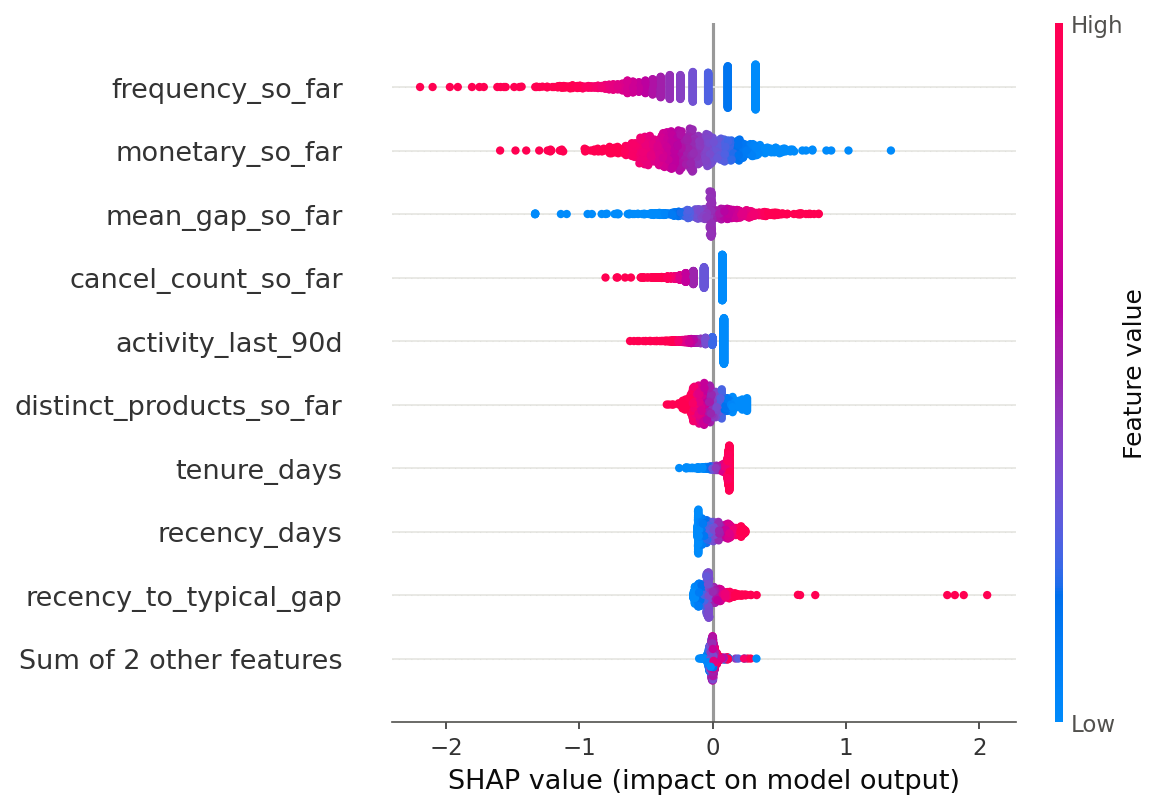
\includegraphics[width=0.85\textwidth]{figures/ch8_shap_summary.png}
\end{center}

By mean absolute SHAP value, the most influential features are \texttt{frequency\_so\_far} and \texttt{monetary\_so\_far} (the two RFM features driving most of the model's separating power, consistent with Sections~\ref{sec:8-3}--\ref{sec:8-5}), followed by \texttt{activity\_last\_90d} and, at a similar level to each other, the cancellation count, the mean inter-purchase gap and tenure. Higher frequency, higher monetary value and more purchases in the last 90 days push the prediction toward \emph{not} churning; a longer typical gap between purchases and a longer tenure push toward churning, and so does being overdue relative to one's own rhythm (\texttt{recency\_to\_typical\_gap}). \texttt{recency\_days} itself has a small weight once recent activity and the recency-to-gap ratio are in the model, because those two features already carry most of its information.

The cancellation count has a \emph{negative} coefficient: holding the other features fixed, customers with more cancellations are slightly \emph{less} likely to churn. Cancellations are a by-product of ordering a lot: the cancellation count has a Spearman correlation of 0.60 with \texttt{frequency\_so\_far}, customers with at least one cancellation have a median of 6 purchase occasions (vs.\ 2 without), and their churn rate is 35.7\% (vs.\ 59.2\%). The count therefore acts as an extra engagement signal. \textbf{These are associations the model has learned, not causal effects} (Section~\ref{sec:3-14}) -- the model does not imply that encouraging cancellations would retain customers.

\section{Training Population Ablation}
\label{sec:8-10}

Compare two training schemes for the selected model (Logistic Regression, Full features, $C=0.01$), both trained on the \textbf{train period only} (not the extended refit pool from Section~\ref{sec:8-7}) and evaluated on the \textbf{same test set}:

\begin{center}
\begin{tabular}{@{}p{4.5cm}p{9.6cm}@{}}
    \toprule
    Scheme & Training rows \\
    \midrule
    A -- Episode (main) & \texttt{in\_training\_sample} rows, unweighted (6,453 rows) \\
    B -- All weekly, weighted & All weekly active rows in the training period, weighted by \texttt{sample\_weight} (61,415 rows) \\
    \bottomrule
\end{tabular}
\end{center}

\begin{center}
\begin{tabular}{@{}p{3.2cm}p{1.8cm}p{1.8cm}p{2.4cm}p{1.8cm}@{}}
    \toprule
    Scheme & ROC-AUC & PR-AUC & Precision@10\% & Lift@10\% \\
    \midrule
    A -- Episode & 0.752 & 0.632 & 0.713 & 1.780 \\
    B -- Weighted all & 0.756 & 0.648 & 0.769 & 1.919 \\
    \bottomrule
\end{tabular}
\end{center}

\textbf{When trained on the train period only, B is better} on every metric, using $9.5\times$ more rows (61,415 vs.\ 6,453): with so few customers and snapshots, discarding the correlated-but-informative extra rows removes some signal along with the redundancy.

\textbf{The advantage shrinks once more training data is available.} After the train + validation refit of Section~\ref{sec:8-7} (12,019 episode rows vs.\ 120,376 weighted rows), Logistic Regression on Scheme B is not significantly better than Scheme A on test (PR-AUC 0.661 vs.\ 0.658; customer-level bootstrap $\Delta$PR-AUC $+0.003$, 95\% CI $[-0.004, +0.010]$; notebook \texttt{08b}). Two details matter for reading the table above: the raw $1/n_i$ weights average 0.064, so with the same $C$ they also make the regularization relatively much stronger under Scheme B; and with weights rescaled to mean 1, Logistic Regression on Scheme B is insensitive to $C$ (validation PR-AUC 0.769--0.770 for $C$ from 0.001 to 10).

The episode scheme (A) therefore remains an acceptable default at this data size: it cuts near-duplicate rows and training time by over 90\% (Section~\ref{sec:6-15}) at no significant cost once the final refit is done. Scheme B is a reasonable alternative and becomes more attractive when the training window is short.


\chapter{Evaluation}
\label{ch:evaluation}
\section{Evaluation Framework}
\label{sec:7-1}

Evaluate the final system on the unseen future test period using three layers: \textbf{Predictive Performance}, \textbf{Targeting Performance} and \textbf{Business Impact Estimation}. Results are reported overall and for the one-time and repeat segments.

All evaluation uses the \textbf{Scoring Population}: every active customer at every weekly test date. Because the historical data contain no campaigns, suppression is not applied in the main evaluation. An optional sensitivity analysis can simulate suppression by removing customers selected in the Top-K during the previous $S$ weeks.

The same customer appears in several consecutive test weeks, so test rows are not independent. This mirrors real operations and is acceptable, but uncertainty is reported across weeks (mean $\pm$ standard deviation) or with a customer-level bootstrap rather than as if rows were independent.

\textbf{Execution.} The final model (Logistic Regression, Full feature set, $C=0.01$) is refit from scratch here using the exact recipe of Section~\ref{sec:6-7} -- trained on the Training Population re-derived over train+validation (12,019 rows) -- rather than loaded from a saved file, so this chapter is self-contained. The test period spans 10 weekly scoring dates (2011-07-04 -- 2011-09-05, Section~\ref{sec:5-9}) and 24,252 Scoring Population rows. Repeat customers make up 86.7\% of test rows and one-time customers 13.3\%; segment-level error rates are reported in Section~\ref{sec:7-12}.

\section{Classification Performance}
\label{sec:7-2}

ROC-AUC, PR-AUC, Precision, Recall and F1. Always report the test churn rate next to PR-AUC as its random reference. \textbf{Calibration} (reliability curve, Brier score) is required whenever probabilities are used as values, e.g.\ expected revenue at risk; Random Forest and XGBoost may need Platt or isotonic calibration fitted on the validation period.

\begin{center}
\begin{tabular}{@{}p{2.6cm}p{1.8cm}p{1.8cm}p{2.4cm}p{1.8cm}p{1.8cm}@{}}
    \toprule
    Test churn rate & ROC-AUC & PR-AUC & Precision@0.5 & Recall@0.5 & F1@0.5 \\
    \midrule
    0.401 & 0.764 & 0.659 & 0.612 & 0.649 & 0.630 \\
    \bottomrule
\end{tabular}
\end{center}

ROC-AUC and PR-AUC match Section~\ref{sec:6-7}'s refit exactly, as expected from the identical recipe. PR-AUC (0.659) sits well above the test churn rate (0.401), its random reference.

\begin{center}
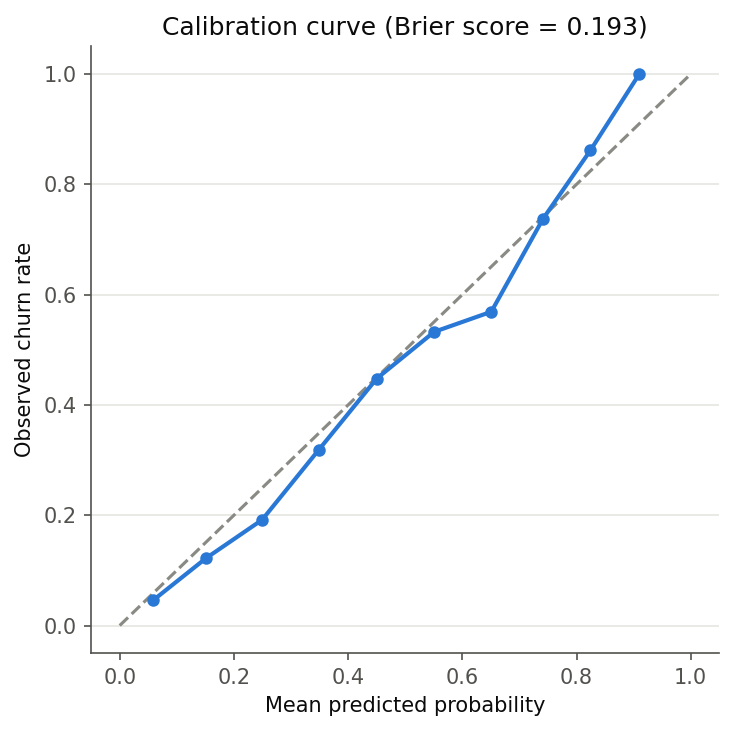
\includegraphics[width=0.55\textwidth]{figures/ch9_calibration_curve.png}
\end{center}

The reliability curve tracks the diagonal reasonably closely (Brier score $= 0.193$), with the model somewhat overestimating risk around predicted probability $\approx 0.65$ (observed churn rate 0.57) and underestimating slightly at the low end -- acceptable for ranking-based targeting, but worth a calibration step (Platt/isotonic) if predicted probabilities are later used directly as values, e.g.\ in Section~\ref{sec:7-5}'s revenue-at-risk estimate.

\section{Ranking Performance}
\label{sec:7-3}

Precision@K, Recall@K, Lift@K and cumulative Gain. Because targeting happens \textbf{each week}, these metrics are computed \textbf{per scoring date} -- rank that week's full Scoring Population, cut the top $K\%$ -- and then summarized as mean $\pm$ standard deviation across test weeks. Pooled curves may be shown additionally but are not the primary result.

At $K=10\%$, computed per week over the 10 test weeks and compared against the recency-rule and RFM-rule baselines (Section~\ref{sec:6-2}) and random targeting:

\begin{center}
\begin{tabular}{@{}p{2.8cm}p{2.6cm}p{2.1cm}p{2.1cm}@{}}
    \toprule
    Candidate & Precision@10\% & Lift@10\% & Gain@10\% \\
    \midrule
    Final model & $0.769 \pm 0.047$ & $1.924 \pm 0.049$ & $0.193 \pm 0.005$ \\
    RFM rule & $0.718 \pm 0.047$ & $1.796 \pm 0.049$ & $0.180 \pm 0.005$ \\
    Recency rule & $0.626 \pm 0.056$ & $1.565 \pm 0.061$ & $0.157 \pm 0.006$ \\
    Random & $0.406 \pm 0.045$ & $1.017 \pm 0.110$ & $0.102 \pm 0.011$ \\
    \bottomrule
\end{tabular}
\end{center}

\begin{center}
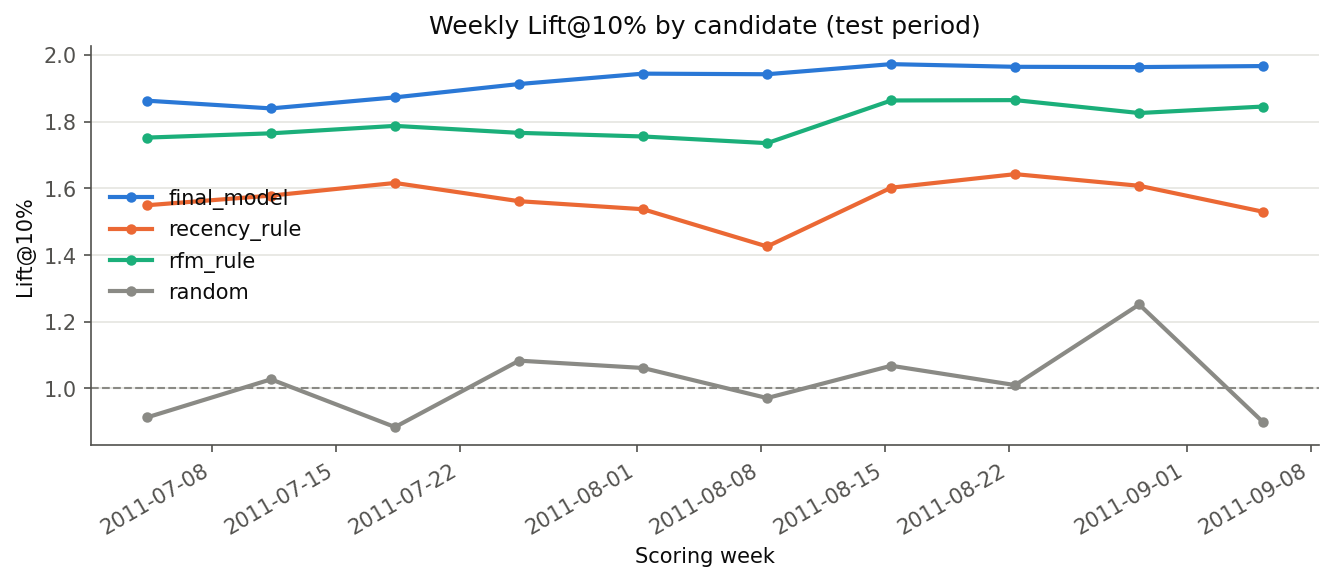
\includegraphics[width=0.85\textwidth]{figures/ch9_weekly_lift.png}
\end{center}

The final model leads every one of the 10 test weeks without exception, and its low week-to-week standard deviation (0.049 on Lift@10\%, versus 0.110 for random) shows the advantage is stable, not a lucky average. \textbf{RFM rule} here is a hand-built, untrained score (recency $-$ frequency $-$ monetary, each standardized on the training period) -- distinct from Section~\ref{sec:6-3}'s \emph{trained} Logistic Regression on the same three features -- and it is the closest competitor to the final model; the recency rule trails both.

\section{Risk Band Analysis}
\label{sec:7-4}

Compare actual churn rates and customer characteristics across risk bands (e.g.\ deciles) to check that higher predicted risk corresponds to higher observed churn.

\begin{center}
\begin{tabular}{@{}p{3cm}p{3cm}p{3cm}@{}}
    \toprule
    Risk decile & Customers & Observed churn rate \\
    \midrule
    1 (lowest) & 2,426 & 5.1\% \\
    3 & 2,425 & 18.6\% \\
    5 & 2,425 & 38.8\% \\
    7 & 2,425 & 53.8\% \\
    8 & 2,425 & 53.5\% \\
    10 (highest) & 2,426 & 77.3\% \\
    \bottomrule
\end{tabular}
\end{center}

Observed churn rate rises almost monotonically from 5.1\% to 77.3\% across deciles -- a 15$\times$ spread confirming the score is informative, not just well-ranked on average. The one exception is decile 8 (53.5\%), marginally below decile 7 (53.8\%); not material given weekly sample sizes.

\section{Customer Revenue at Risk}
\label{sec:7-5}

Estimate potential future revenue associated with churners, using a customer-level proxy:
\begin{align*}
    \text{AvgPurchaseValue}_i &= \text{TotalRevenue}_i \div \text{PurchaseOccasions}_i \\
    \text{RevenueAtRisk}_i &= \text{AvgPurchaseValue}_i \quad \text{(one future purchase-equivalent)}
\end{align*}
or, with enough history:
\begin{equation*}
    \text{RevenueAtRisk}_i = \text{AvgMonthlyRevenue}_i \times H \div 30
\end{equation*}
All inputs use history up to the snapshot date only. These are estimates of revenue exposure, not observed lost revenue.

\textbf{Applied here.} The first (proxy) form is used, with \texttt{avg\_order\_value\_so\_far} (Section~\ref{sec:5-6}) standing in for $\text{AvgPurchaseValue}_i$ -- there is not enough post-snapshot history in this $\approx$2-year dataset to estimate a stable $\text{AvgMonthlyRevenue}_i$ for the second form.

\begin{center}
\begin{tabular}{@{}p{2.3cm}p{2.3cm}p{2.3cm}p{2.3cm}p{2.3cm}@{}}
    \toprule
    Mean & Median & Std & Min & Max \\
    \midrule
    395.70 & 303.58 & 561.61 & 2.90 & 14,844.77 \\
    \bottomrule
\end{tabular}
\end{center}

Revenue at risk is as right-skewed as the underlying order-value distribution (Section~\ref{sec:4-6}) -- a small number of high-value customers carry disproportionate weight in the business-impact totals that follow.

\section{Business Impact Scenario}
\label{sec:7-6}

For each target share $K \in \{10, 20, 30, 40, 50\%\}$, per scoring week: customers targeted ($N_K$), true churners captured ($TP_K$), non-churners targeted ($FP_K$), Recall@K, and revenue at risk among targeted churners.

At $K=10\%$, summed across the 10 test weeks (so $N_K$ counts weekly targeting instances, not unique customers -- the same customer can be targeted in more than one week):

\begin{center}
\begin{tabular}{@{}p{2.8cm}p{1.6cm}p{1.6cm}p{1.6cm}p{2.8cm}@{}}
    \toprule
    Candidate & $N_K$ & $TP_K$ & $FP_K$ & Revenue at risk \\
    \midrule
    Final model & 2,427 & 1,867 & 560 & 337,903.72 \\
    RFM rule & 2,427 & 1,743 & 684 & 498,060.34 \\
    Recency rule & 2,427 & 1,521 & 906 & 538,397.09 \\
    Random & 2,427 & 986 & 1,441 & 330,372.57 \\
    \bottomrule
\end{tabular}
\end{center}

$N_K$ is identical across candidates by construction (same $K$, same weekly population); $TP_K$ and revenue at risk are not -- the final model captures the most churners, but the two baselines happen to target higher-average-order-value customers, so they show \emph{more} revenue at risk despite capturing fewer churners. This tension carries through to Sections~\ref{sec:7-9}--\ref{sec:7-10}.

\section{Retention Effectiveness Assumption}
\label{sec:7-7}

Retention success is an assumption, not an observed result. Scenarios: \textbf{Conservative $e = 30\%$}, \textbf{Base $e = 40\%$}, \textbf{Optimistic $e = 50\%$}.
\begin{equation*}
    \text{RevenuePreserved} = \text{RevenueAtRisk(targeted churners)} \times e
\end{equation*}

At $K=10\%$ (Section~\ref{sec:7-6}'s targeted churners), revenue preserved across the three effectiveness scenarios:

\begin{center}
\begin{tabular}{@{}p{2.8cm}p{2.6cm}p{2.6cm}p{2.6cm}@{}}
    \toprule
    Candidate & $e=30\%$ & $e=40\%$ (Base) & $e=50\%$ \\
    \midrule
    Final model & 101,371.12 & 135,161.49 & 168,951.86 \\
    RFM rule & 149,418.10 & 199,224.14 & 249,030.17 \\
    Recency rule & 161,519.13 & 215,358.84 & 269,198.55 \\
    Random & 99,111.77 & 132,149.03 & 165,186.28 \\
    \bottomrule
\end{tabular}
\end{center}

Because revenue preserved scales linearly with $e$ for a fixed set of targeted churners, the ranking across candidates is unchanged by the effectiveness assumption -- only Section~\ref{sec:7-9}'s cost terms can shift it.

\section{Marketing Cost and the Value of the Model}
\label{sec:7-8}

If contact cost per customer is roughly constant, targeting $K\%$ instead of everyone reduces reach cost by $(1 - K)$. This saving comes from \textbf{targeting itself}, not from the model -- any ranking at the same $K$ saves the same amount.

The model's contribution is measured by comparing, \textbf{at the same $K$}, the churners captured, revenue preserved and net impact of:
\begin{enumerate}
    \item the final model,
    \item the recency-rule baseline, and
    \item random targeting.
\end{enumerate}

At $K=10\%$, $e=40\%$ (Base), contact cost is identical across candidates by construction ($N_K \times c_{\text{contact}}$, same $N_K$):

\begin{center}
\begin{tabular}{@{}p{2.8cm}p{3cm}p{3cm}p{2.6cm}@{}}
    \toprule
    Candidate & Customers targeted & Churners captured & Contact cost \\
    \midrule
    Final model & 2,427 & 1,867 & 1,213.50 \\
    RFM rule & 2,427 & 1,743 & 1,213.50 \\
    Recency rule & 2,427 & 1,521 & 1,213.50 \\
    Random & 2,427 & 986 & 1,213.50 \\
    \bottomrule
\end{tabular}
\end{center}

The reach-cost saving from targeting 10\% instead of everyone is the same 1,213.50 regardless of which candidate ranks customers -- confirming it comes from \emph{targeting}, not the model. The model's own contribution shows up only in churners captured (1,867 vs.\ 986 for random, almost double) -- whether that translates into more net business value depends on revenue at risk and incentive cost too (Section~\ref{sec:7-9}).

\section{Net Business Impact}
\label{sec:7-9}

Because preserved revenue is not profit, a margin assumption converts it before subtracting costs:
\begin{align*}
    \text{GrossProfitPreserved} &= \text{RevenuePreserved} \times m \\
    \text{ContactCost} &= N_K \times c_{\text{contact}} \\
    \text{IncentiveCost} &= (TP_K \times e + FP_K \times r) \times c_{\text{inc}} \\
    \text{NetBusinessImpact} &= \text{GrossProfitPreserved} - \text{ContactCost} - \text{IncentiveCost}
\end{align*}
Here $r$ is the assumed share of targeted non-churners who redeem an incentive although they would have purchased anyway (cannibalization). Optionally report $\text{GrossProfitPreserved} \div (\text{ContactCost} + \text{IncentiveCost})$.

At $K=10\%$, $e=40\%$ (Base), $m=35\%$, $c_{\text{contact}}=\pounds0.50$, $c_{\text{inc}}=\pounds5.00$, $r=20\%$:

\begin{center}
\footnotesize
\setlength{\tabcolsep}{3pt}
\begin{tabular}{@{}p{2.2cm}p{1.3cm}p{1.3cm}p{1.6cm}p{1.9cm}p{1.6cm}p{1.6cm}p{1.9cm}@{}}
    \toprule
    Candidate & $TP_K$ & $FP_K$ & Revenue preserved & Gross profit preserved & Contact cost & Incentive cost & Net impact \\
    \midrule
    Final model & 1,867 & 560 & 135,161.49 & 47,306.52 & 1,213.50 & 4,294.00 & \textbf{41,799.02} \\
    RFM rule & 1,743 & 684 & 199,224.14 & 69,728.45 & 1,213.50 & 4,170.00 & 64,344.95 \\
    Recency rule & 1,521 & 906 & 215,358.84 & 75,375.59 & 1,213.50 & 3,948.00 & \textbf{70,214.09} \\
    Random & 986 & 1,441 & 132,149.03 & 46,252.16 & 1,213.50 & 3,413.00 & 41,625.66 \\
    \bottomrule
\end{tabular}
\end{center}

\textbf{Counter-intuitive result.} At this operating point, the \emph{final model's net business impact is the lowest of the three learned/rule-based candidates} -- even below the simple recency rule -- despite capturing the most churners and leading every predictive and ranking metric in this chapter. The reason is visible in Section~\ref{sec:7-6}: revenue at risk is driven by \emph{which} customers are targeted (their average order value), not by how many churners are caught. The recency and RFM rules happen to target a higher-order-value subset of customers, so they preserve more revenue per targeted churner even while catching fewer of them. This is not a bug in the model -- it optimizes churn-probability ranking, not revenue-weighted ranking -- but it means \textbf{the best classifier is not automatically the best business decision at a fixed $K$}, a central caveat for Sections~\ref{sec:7-10}--\ref{sec:7-11}.

\section{Scenario Analysis}
\label{sec:7-10}

Present a business-impact table across $K$ and $e$, with $m$, $c_{\text{contact}}$, $c_{\text{inc}}$ and $r$ stated explicitly:

For the final model, with $m$, $c_{\text{contact}}$, $c_{\text{inc}}$ and $r$ held at Section~\ref{sec:7-9}'s assumptions; ``Net impact'' and the comparison column use $e=40\%$ (Base):

\begin{center}
\footnotesize
\setlength{\tabcolsep}{3pt}
\begin{tabular}{@{}p{0.9cm}p{1.3cm}p{1.5cm}p{1cm}p{2.3cm}p{2.4cm}p{1.6cm}p{1.7cm}p{1.8cm}@{}}
    \toprule
    Target \% & Customers & Churners captured & Recall\newline @K & Revenue at risk & Preserved (30/40/50\%) & Costs & Net impact & Net impact vs recency rule \\
    \midrule
    10\% & 2,427 & 1,867 & 0.19 & 337,903.72 & 101,371 / 135,161 / 168,952 & 5,507.50 & 41,799.02 & $-$28,415.07 \\
    20\% & 4,850 & 3,377 & 0.35 & 794,130.67 & 238,239 / 317,652 / 397,065 & 10,652.00 & 100,526.29 & $-$32,792.34 \\
    30\% & 7,274 & 4,697 & 0.48 & 1,356,293.83 & 406,888 / 542,518 / 678,147 & 15,608.00 & 174,273.14 & $-$18,504.64 \\
    40\% & 9,700 & 5,993 & 0.62 & 1,878,460.72 & 563,538 / 751,384 / 939,230 & 20,543.00 & 242,441.50 & $-$5.62 \\
    50\% & 12,126 & 7,148 & 0.74 & 2,412,837.41 & 723,851 / 965,135 / 1,206,419 & 25,337.00 & 312,460.24 & $+$26,781.55 \\
    \bottomrule
\end{tabular}
\end{center}

Widening $K$ increases both Recall@K and net impact monotonically for the final model, but the comparison to the recency rule only turns positive between $K=30\%$ and $K=40\%$ (crossing almost exactly at $K=40\%$, where the gap is $-\pounds5.62$, essentially a wash), and becomes clearly favorable only at $K=50\%$ ($+\pounds26,781.55$). At the narrow targeting shares most realistic for a retention campaign ($K=10$--$30\%$), the model trails the simple recency rule on net business impact, reinforcing Section~\ref{sec:7-9}'s caveat.

\section{Model Comparison}
\label{sec:7-11}

Compare candidates (including baselines) on predictive metrics, ranking metrics, calibration, operational targeting capacity and business-impact scenarios. Do not define a single "best" model from classification metrics alone when the objective depends on ranking and cost constraints.

\begin{center}
\begin{tabular}{@{}p{2.8cm}p{1.6cm}p{1.6cm}p{2.8cm}p{2.8cm}@{}}
    \toprule
    Candidate & ROC-AUC & PR-AUC & Weekly Lift@10\% & Net impact ($K$=10\%, $e$=40\%) \\
    \midrule
    Final model & 0.764 & 0.659 & $1.924 \pm 0.049$ & 41,799.02 \\
    RFM rule & 0.736 & 0.624 & $1.796 \pm 0.049$ & 64,344.95 \\
    Recency rule & 0.638 & 0.531 & $1.565 \pm 0.061$ & 70,214.09 \\
    Random & 0.506 & 0.404 & $1.017 \pm 0.110$ & 41,625.66 \\
    \bottomrule
\end{tabular}
\end{center}

No candidate wins on every column. The final model is unambiguously best on predictive and ranking metrics (ROC-AUC, PR-AUC, Lift@10\% and its stability) -- against the Success Criteria of Section~\ref{sec:2-6}, it clears the ``PR-AUC/Lift beat the baselines'' bar comfortably. But the rule-based baselines preserve more net business value at the default $K=10\%$ operating point (Section~\ref{sec:7-9}), so the ``business-scenario'' success criterion is not met at that $K$ -- only from $K\approx40\%$ upward (Section~\ref{sec:7-10}). This gap between predictive quality and business outcome, not any single metric, is the main input to the deployment recommendation (Chapter~\ref{ch:deployment}).

\section{Error Analysis and Limitations}
\label{sec:7-12}

Investigate false positives, false negatives, segments (one-time vs repeat, UK vs non-UK, wholesale-sized customers) and weeks where performance differs, including seasonal effects. State clearly that Online Retail II contains no campaign treatment/control information, so incremental revenue, causal retention effect and true campaign ROI cannot be identified. Business-impact results are scenario estimates.

Targeting the top 10\% by the final model's score, pooled across the test period: 57.7\% true negatives, 32.3\% false negatives, 7.7\% true positives, 2.3\% false positives -- the false-negative share is large by construction, since a 10\%-wide net cannot catch most of a $\approx$40\% base rate.

\begin{center}
\begin{tabular}{@{}p{3.6cm}p{2.6cm}p{2.6cm}@{}}
    \toprule
    Group & FP rate (among targeted) & FN rate (among non-targeted) \\
    \midrule
    One-time & 20.6\% & 55.5\% \\
    Repeat & 25.3\% & 34.1\% \\
    \midrule
    UK & 22.3\% & 36.3\% \\
    Non-UK & 29.4\% & 32.5\% \\
    \midrule
    Retail & 22.7\% & 37.2\% \\
    Wholesale-like & n/a (0 targeted) & 7.8\% \\
    \bottomrule
\end{tabular}
\end{center}

Three patterns stand out. \textbf{One-time customers} are missed far more often than repeat customers (55.5\% vs.\ 34.1\% FN rate) -- with only one purchase occasion, their feature history is thin, and the model has less signal to work with (consistent with the One-time group of Section~\ref{sec:4-6}). \textbf{Non-UK customers} see a higher false-positive rate (29.4\% vs.\ 22.3\% for UK) -- the model, trained overwhelmingly on UK behavior (Section~\ref{sec:4-2}), generalizes a little less cleanly to the small non-UK population. \textbf{Wholesale-like customers} (top 1\% by revenue so far) are the model's strongest case: a 7.8\% false-negative rate, far below retail's 37.2\%, and none were false positives in the targeted top 10\% -- their high, frequent purchase volume makes their churn signal unusually clear.

\textbf{Principle.} \textbf{Project-wide business-impact principle.} The model identifies and prioritizes churn risk; the retention campaign determines treatment; actual incremental revenue requires treatment/control data. Revenue at risk, revenue preserved, cost saving and net impact are simulation outputs unless supported by observed campaign outcomes.


\chapter{Deployment}
\label{ch:deployment}
\textbf{Note.} This chapter describes a \textbf{proposed operational design}. It is not implemented as a live system in this project.

\section{Deployment Objective}
\label{sec:8-1}

Provide recurring churn scoring that produces a prioritized existing-customer population for retention marketing.

\section{Weekly Batch Pipeline}
\label{sec:8-2}

The training-episode cooldown is \textbf{not} part of this pipeline; it exists only in training-data construction.

\begin{center}
\textbf{Latest transactions} $\rightarrow$ \textbf{Valid transactions} $\rightarrow$ \textbf{Active customers} (Recency $\leq R_{\max}$) $\rightarrow$ \textbf{Remove suppressed customers} \\[0.3cm]
$\rightarrow$ \textbf{Snapshots} $\rightarrow$ \textbf{Features} $\rightarrow$ \textbf{Scoring} $\rightarrow$ \textbf{Ranking} $\rightarrow$ \textbf{Capacity \& business rules} $\rightarrow$ \textbf{Target population}
\end{center}

\section{Customer Risk Output}
\label{sec:8-3}

Minimum output: \texttt{customer\_id}, \texttt{snapshot\_date}, \texttt{churn\_probability}, \texttt{risk\_band}, \texttt{rank}, \texttt{segment}, \texttt{model\_version}.

\section{Target Population}
\label{sec:8-4}

Select target customers based on churn risk, marketing capacity and business constraints.

\section{Suppression}
\label{sec:8-5}

Customers \textbf{contacted} in a campaign are excluded from the Scoring Population for a configurable suppression period $S$ (e.g.\ 4--8 weeks), so they are not targeted repeatedly. Suppression:

\begin{itemize}
    \item applies only to customers who were actually targeted, not to everyone who was scored;
    \item is an operational business rule, independent of the training-episode cooldown $C$;
    \item is logged, so that suppressed customers can be analyzed separately once campaign data exist.
\end{itemize}

\section{Monitoring}
\label{sec:8-6}

Data quality, feature drift, model performance, calibration, lift, risk-band behavior and business metrics where available.


\chapter{Feedback}
\label{ch:feedback}
\textbf{Note.} Like Chapter~\ref{ch:deployment}, this chapter is a \textbf{proposed design}.

\section{Feedback Loop}
\label{sec:9-1}

After $H$ days, observe customer purchases and compare predicted churn with actual churn.

\section{Model Performance Monitoring}
\label{sec:9-2}

Track classification and weekly Top-K ranking metrics over time.

\section{Business Outcome Monitoring}
\label{sec:9-3}

Track repurchase rate, revenue contribution, target population and campaign cost when available.

\section{Data Drift}
\label{sec:9-4}

Monitor transaction volume, feature distributions and customer behavior.

\section{Concept Drift}
\label{sec:9-5}

Monitor changes in the relationship between behavior and future churn, including seasonal shifts.

\section{Campaign Feedback}
\label{sec:9-6}

If treatment/control data become available, evaluate campaign response and incremental outcomes; this would also allow the assumed $e$, $r$ and costs to be replaced by measured values.

\section{Model Retraining}
\label{sec:9-7}

Retrain periodically or when performance, drift or behavior changes justify it, using the same embargoed temporal design and the same Training Population rule.


\chapter{Conclusion}
\label{ch:conclusion}
\section{Summary of Strategy}
\label{sec:12-1}

The project connects e-commerce revenue generation with customer retention and churn prediction. Repeat customers are 72.3\% of the customer base but generate 96.7\% of revenue (Section~\ref{sec:6-8}), so keeping existing customers buying is where almost all revenue already is. The project therefore predicts, every week, which active customers are likely to make no purchase in the next 90 days, so that a retention campaign with limited capacity can be pointed at them first.

\section{Business-to-Technical Translation}
\label{sec:12-2}

The business objective is to increase sales revenue through repeat-purchase revenue from existing customers while controlling retention and marketing cost. The technical solution is customer-level churn prediction and risk ranking:

\begin{itemize}
    \item \textbf{Unit of analysis:} one row per Customer $\times$ weekly snapshot date, with features computed only from history up to that date (208,764 rows, Chapter~\ref{ch:data-preparation}).
    \item \textbf{Label:} churn $=1$ if the customer makes no valid purchase in the next $H = 90$ days; only customers active in the last $R_{\max} = 136$ days are scored.
    \item \textbf{Evaluation:} a chronological train / validation / test split with 90-day embargoes, so that no label used for training overlaps the period it is evaluated on (Section~\ref{sec:7-9}).
    \item \textbf{Decision:} rank each week's active customers by predicted churn probability and contact the top $K\%$ that the campaign budget allows.
\end{itemize}

\section{Key Results}
\label{sec:12-3}

\textbf{Answers to the research questions} (Section~\ref{sec:1-4}):

\begin{enumerate}
    \item \textbf{From transactions to observations.} 1,067,371 raw transaction lines become 776,577 valid lines, 36,594 purchase occasions and a weekly table of 208,764 leakage-checked Customer $\times$ Snapshot rows with 11 point-in-time features. Two automatic checks guard the construction: no feature is sourced from after its snapshot date, and recent activity is consistent with recency and frequency on every row.
    \item \textbf{How well behavior predicts churn.} On the unseen test period (July--September 2011, churn rate 40.1\%), the final model -- Logistic Regression on the full feature set -- reaches ROC-AUC 0.765 and PR-AUC 0.658. A tuned XGBoost is not meaningfully better (Section~\ref{sec:8-6}), which indicates that the signal in these features is close to additive and monotone.
    \item \textbf{Prioritization under limited capacity.} Contacting the top 10\% of each week's ranking reaches churners 1.90 times as often as random contact (76\% of contacted customers are churners, versus 41\% at random), and beats both simple rules: an RFM score (Lift 1.80) and recency alone (Lift 1.57). The model leads in every one of the 10 test weeks.
    \item \textbf{Behavior associated with churn.} Fewer purchases so far, lower cumulative spending and fewer purchases in the last 90 days go with a higher churn risk; a longer typical gap between purchases and being overdue relative to one's own rhythm go with a higher risk. These are associations, not causes (Section~\ref{sec:8-9}).
\end{enumerate}

\textbf{Comparison of targeting strategies} on the test period (weekly averages; net impact under the base scenario of Section~\ref{sec:9-9}: retention effectiveness 40\%, margin 35\%, contact cost \pounds0.50, incentive \pounds5):

\begin{center}
\footnotesize
\begin{tabular}{@{}lcccc@{}}
    \toprule
    Strategy & PR-AUC & Lift@10\% & Churners reached (10 weeks) & Net impact at 10\% (\pounds) \\
    \midrule
    Random & 0.404 & 1.02 & 986 & 41,626 \\
    Recency rule & 0.531 & 1.57 & 1,521 & \textbf{70,214} \\
    RFM rule & 0.624 & 1.80 & 1,743 & 64,345 \\
    Machine-learning model & \textbf{0.658} & \textbf{1.90} & \textbf{1,846} & 42,388 \\
    \bottomrule
\end{tabular}
\end{center}

\textbf{Against the success criteria} (Section~\ref{sec:2-7}):

\begin{center}
\small
\begin{tabular}{@{}p{3.1cm}p{9.2cm}p{1.9cm}@{}}
    \toprule
    Criterion & Result on the test period & Met? \\
    \midrule
    Predictive & PR-AUC 0.658, above the churn rate (0.401) and the recency rule (0.531). & Yes \\
    Targeting & At $K = 20\%$ and $30\%$, weekly Lift 1.74 and 1.62 (recency rule 1.44 and 1.37); weekly Recall 0.35 and 0.49 (recency rule 0.29 and 0.41). & Yes \\
    Stability & The model leads the baselines in all 10 test weeks; weekly Lift@10\% $1.90 \pm 0.06$. & Yes \\
    Business scenario & Net impact is positive at every $K$, but below the recency rule up to $K = 40\%$; it is higher only at $K = 50\%$ (+\pounds30,142). & No (only at $K = 50\%$) \\
    \bottomrule
\end{tabular}
\end{center}

\textbf{The central lesson} is that the best classifier is not automatically the best business decision. The model finds the most churners, but many of them are small, one-time buyers with low order values, whereas the recency rule happens to pick customers who spend more per order. Because the simulated value of retaining a customer is proportional to their order value, a better churn ranking does not translate into more preserved revenue at a small $K$ (Section~\ref{sec:9-9}).

\section{Operational Strategy}
\label{sec:12-4}

Weekly batch scoring of all active customers, customer snapshots, episode-based sampling for training, suppression of contacted customers, churn prediction, ranking and Top-K targeting. Given the results above, the recommended use is:

\begin{itemize}
    \item Use the model's ranking to decide \emph{who is likely to churn}, and combine it with customer value when deciding \emph{who is worth an incentive}: for example, rank by expected loss (churn probability $\times$ average order value), or reserve costly incentives for high-value customers in the top risk bands and use a low-cost channel (automated e-mail) for low-value ones.
    \item Choose $K$ from the campaign budget, not from the model; report Lift and Recall at that $K$ every week, alongside the recency rule as a running benchmark.
    \item Suppress contacted customers for a few weeks and keep a random hold-out group that is not contacted, so that the real effect of the campaign can be measured later (Chapter~\ref{ch:feedback}).
\end{itemize}

\section{Limitations}
\label{sec:12-5}

\begin{itemize}
    \item \textbf{No campaign data.} The dataset lacks marketing treatment, cost, margin and control-group information, so causal uplift, incremental revenue and true ROI cannot be established. All revenue and profit figures are scenario estimates under stated assumptions.
    \item \textbf{Short history and seasonality.} The $\sim$2-year span gives only 10 test weeks (July--September 2011). The test period does not include the October--December peak, whose behavior differs most (churn rates of 60\% and more for December snapshots), and churn rates differ markedly between train (43.0\%), validation (52.9\%) and test (40.1\%).
    \item \textbf{One-time buyers.} With only one purchase in their history, these customers are much harder to rank (ROC-AUC 0.657 vs.\ 0.759 for repeat customers; 56.0\% of the one-time customers left outside the top 10\% go on to churn, vs.\ 34.3\% for repeat customers, Section~\ref{sec:9-12}).
    \item \textbf{Fixed design choices.} $R_{\max}$ and $H$ were chosen from the full dataset rather than from the training period alone (Section~\ref{sec:7-8}).
\end{itemize}

\section{Future Work}
\label{sec:12-6}

\begin{itemize}
    \item Integrate campaign and financial data, run treatment/control experiments, and move from churn prediction to uplift modeling (who changes behavior \emph{because} of a contact).
    \item Make the ranking value-aware (expected loss, or a model of future spend) and evaluate it with the same business-impact chain.
    \item Add features aimed at one-time buyers (first-order basket, product category, country, time of year) or treat them with a separate model.
    \item Extend the test period to cover a full year, including the year-end peak, and retrain on a rolling window.
\end{itemize}


\end{document}
